\documentclass{book}

\usepackage{graphicx}

\usepackage{hyphenat} % http://www.ctex.org/documents/packages/special/hyphenat.pdf

\usepackage{setspace}\onehalfspacing\frenchspacing\flushbottom\sloppy

% https://www.scivision.dev/include-svg-vector-latex/
%\usepackage{svg}
% see https://tex.stackexchange.com/questions/442077/is-it-possible-to-use-svg-images-with-overleaf

% https://tex.stackexchange.com/a/8459/235813
\usepackage[nottoc]{tocbibind}

\usepackage{hyperref}
\hypersetup{
    colorlinks=true,
    linkcolor=blue,
    filecolor=magenta,      
    urlcolor=cyan,
    pdftitle={Overleaf Example},
    pdfpagemode=FullScreen,
    }

% https://en.wikibooks.org/wiki/LaTeX/Glossary says
% "\usepackage{glossaries} and \makeglossaries in your preamble (after \usepackage{hyperref} if present)"

% https://www.overleaf.com/learn/latex/Glossaries
\usepackage[toc]{glossaries}

\makeglossaries % The command must be before the first glossary entry.

% https://en.wikibooks.org/wiki/LaTeX/Glossary says
% "define any number of \newglossaryentry and \newacronym glossary and acronym entries in your preamble"
% see https://en.wikibooks.org/wiki/LaTeX/Glossary
% and https://www.overleaf.com/learn/latex/Glossaries

\newglossaryentry{organization}{
  name={organization},
  plural={organizations},
  description={an assembly of teams. The name of the concept might be a corporation, an agency, a department, a bureau, or any other aggregation of smaller organizations}
}

\newglossaryentry{culture}{
name={culture},
plural={cultures},
description={norms, expectations around interaction among people}
}

\newglossaryentry{stakeholder}{
name={stakeholder},
plural={stakeholders},
description={a person who cares about the process or the outcome; distinct from a participant}
%descriptionplural={people who cares about the process or the outcome; distinct from participants}
}

\newglossaryentry{participant}{
name={participant},
description={a person who is expected to take action or make contribution}
}

\newglossaryentry{essential bureaucracy}{
name={essential bureaucracy},
text={Essential bureaucracy},
description={the minimum processes and staffing and skills necessary to address the complexity of the problem space}
}

\newglossaryentry{bureaucratic debt}{
name={bureaucratic debt},
plural={bureaucratic debts},
text={Bureaucratic debt},
description={the cost of work need to change a process caused by choosing an easy solution now instead of using a better approach that would take longer}
}

\newglossaryentry{subject}{
    name={subject},
    plural={subjects},
    description={the person experiencing bureaucracy}
}
\newglossaryentry{Prisoner's dilemma}{
    name={Prisoner's dilemma},
    description={Two or more people with incomplete information of a situation will make suboptimal choices compared to someone with perfect knowledge of the situation}
}

\newglossaryentry{thought terminating}{
name={thought terminating},
description={\href{https://en.wikipedia.org/wiki/Thought-terminating_clich\%C3\%A9}{thought terminating statements} initially sound reasonable but, upon reflection and analysis, are incorrect}
}

\newglossaryentry{presence creates priority}{
name={presence creates priority},
description={being physically at a person's desk motivates that person to respond better than calling them or emailing them}
}

% https://graphthinking.blogspot.com/2021/07/bureaucracy-book-outline.html
\newglossaryentry{bureaucrat}{
    name={bureaucrat},
    plural={bureaucrats},
    description={the person who is a member of an organization and is responsible for subjective implementation of policy for the organization. Conventional examples of a bureaucrat role: teacher, police, government employee}
}

\newglossaryentry{simple decision}{
  name={simple decision},
  description={has one correct or beneficial choice and one or more wrong or harmful choices.}
}

% https://tex.stackexchange.com/questions/69567/uppercase-word-in-glossary-lowercase-in-text
\newglossaryentry{bureaucracy}{
    name={bureaucracy},
    plural={bureaucracies},
    text={bureaucracy},
    description={
    An organization of bureaucrats comprises a bureaucracy. A bureaucracy facilitates coordination of stakeholders. 
    Bureaucracy is how large organizations make distributed decisions using distributed knowledge.    \\
    Everything in a bureaucracy is made up by other participants. \\
    Bureaucracy is a macroscopic phenomenon emergent at sufficient scale. The scale is important because there is no longer dependence on individual relationships. \\
    Bureaucracy arises when there is no common objectively quantifiable feedback mechanism for individual participants in the organization.\\
    Bureaucracy is a wicked problem}
}

\newglossaryentry{visible bureaucracy}{
name={visible bureaucracy},
    %name={bureaucracy, visible},
    description={procedures and processes are written down and can be discovered by stakeholders}
}
\newglossaryentry{invisible bureaucracy}{
name={invisible bureaucracy},
    %name={bureaucracy, invisible},
    description={procedures and processes are known to some stakeholders and are conveyed verbally to some of the other stakeholders}
}

\newglossaryentry{process}{
name={process},
plural={processes},
description={a task broken into a specified set of subtask dependencies}
}



\title{How to be an Effective Bureaucrat\\
A Guidebook for Everyone}
\author{Ben Payne}
\date{\today}

\begin{document}

\begin{titlepage}
\maketitle
\thispagestyle{empty}
\end{titlepage}
\newpage

%\thispagestyle{empty}
\frontmatter % the front of the book has roman numerals

%\pagenumbering{gobble}
\thispagestyle{empty}

Copyright \copyright 2022 Ben Payne

\ \\

\href{https://creativecommons.org/licenses/by-nc/4.0/}{Creative Commons Attribution-NonCommercial 4.0 International License}
\clearpage
\thispagestyle{empty}

Thank you to my coworkers. Our interactions me learn how to be a better bureaucrat.%\clearpage
%\pagenumbering{roman}

\chapter*{Foreword}% * excludes from Contents)

% Who this book is for

%If you don't think of yourself as a bureaucrat, I hope to change your mind on this essential topic. 
If you have a negative impression of bureaucracy, I want to convince you that bureaucracy is vital and that you can learn to skillfully navigate bureaucracy.

I see this struggle of bureaucracy as critical to modern society. The challenge of bureaucracy is widespread across a variety of governments in different societies, and bureaucracy is durable -- it has existed for hundreds if not thousands of years. Therefore, tackling the challenge of bureaucracy is exciting for me. I enjoy pondering hard problems and then leveraging insights gained from reflection. Being an effective bureaucrat is important to me because bureaucracy can be a force multiplier beyond what I could accomplish on my own.

% from https://graphthinking.blogspot.com/2021/07/bureaucracy-book-outline.html
This book is for you if you are curious about the complex world we live in, or you are thinking about how to productively contribute to society, or you want impactful employment, or your job is not what you expected. If you're wondering why innovation is hard within a bureaucratic organization, this guidebook is intended to help understand what the challenges are.


% What you should expect reading this book: 
Everyone in modern society is a participant in bureaucracy. The purpose of this book is to decrease the surprise of that experience and better arm you emotionally and intellectually for the toil of being a bureaucrat. With focused reflection and a good guidebook, you can improve your skills as a bureaucrat. 

This book is neither a defense of bureaucracy, nor is it intended to disparage bureaucrats or the system of bureaucracy. Instead, the intent of this book is to serve as a guide to bureaucracy-as-it-is. 

This book does not focus on leadership, managing a team, being a team member, planning, time management, project management, advancing your career, or self-improvement. However, in the process of being a better bureaucrat some lessons may apply in those domains.

This book doesn't address personal stress caused by bureaucracy, how to decrease stress, or how to balance the activities of work and life-outside-work. 

This book doesn't focus on citizens, Congress (state or federal), or competing organizations. 

This book doesn't address discrimination or harassment. This book doesn't address bad coworkers, abusive bosses, psychological defects of individuals, or malicious intent. Issues like lying, bribery, and criminal behavior are not discussed. All these aspects happen whenever people interact; the challenges are not specific to bureaucracy. In this book I assume you are honest, and that other people are honest. Even with this simplifying assumption the complexities of bureaucracy arise. In the context of that benign bureaucracy, guidance on how to be an effective bureaucrat is provided.


% What is the benefit of reading this book?
As a result of reading this book, you will be better able to recognize and navigate complex professional environments, both within your career and outside of work. The perspectives offered in this book can benefit you directly, whether by promotion of title, increase in pay, successful completion of a project, or through decreased stress of understanding how the world operates. Being a more effective bureaucrat can also positive impact the causes you care about and the people you engage with.

If you do not recognize that you are bureaucrat, you won't know what is your own fault, the fault of your coworkers, the fault of management, and what is intrinsic to bureaucracy. 

If you do not recognize that you are bureaucrat, you're less likely to be successful interacting with those around you. The self-recognition of being a bureaucrat matters; how you behave and what you think your responsibilities are depend on how you label yourself.

Even people who are smart (e.g., they know history, they have memorized capital cities, they can do math) can struggle in the face of complex large-scale systems. Thinking about complex large-scale systems is not part of the education curriculum. This book will help you learn about bureaucracy and lead to an increase of your ability to identify patterns and apply relevant techniques.

% there's no avoiding the issue
Everyone is a bureaucrat because there are no alternatives to bureaucracy for a society. Gaining skills in navigating bureaucracy are helpful both for your own happiness and the well-being of a functioning society. 

Hoping that modern technology will eliminate or reduce bureaucracy is not helpful. Automation and computers merely obfuscate processes and make negotiation more challenging. 

Simplifying interactions with other people to ``this is characterized merely as human relations" is an easier perspective compared to considering bureaucracy as a complex system. 
% this is also stated on page 24 of \cite{1991_Wilson}
However, a simplified view either misses emergent phenomena or mischaracterizes the situation. In either case, your effectiveness is harmed.



% my experience
% I wrote this book for a younger version of me.
 When I first started my job in a large organization I recognized differences between the expectations of the education system I had left and the challenges of a professional environment. Over the years I learned from my mistakes by reflecting on my (in)actions and the consequences. This approach has been an expensive education. My mistakes delayed progress and damaged relationships. The motive in this book is to provide generalizations from my experiences which might benefit the reader.


% Caveats

In my reflections and attempting to draw lessons there is a risk of overanalysis. Sometimes a situation is merely happenstance, and sometimes attempting to extract lessons from randomness is folly. Avoiding conjecture about conspiracy and malice is a fuzzy boundary when insufficient information is available. 

My experiences cannot be generalized to every situation. Some of the observations here may be analogous to your context if you squint. 

Nothing in this book is domain specific, nothing is tied to engineering of products, and nothing is applicable solely in science research or policy development. While this material is intended to be timeless and generic, it is culturally specific to the United States of America in the early twenty first century. There are cultural blindspots not addressed in this book because I did not encounter systemic hurdles in my career as financially privileged white male. 

% Source of this content: 
This material is based on personal experience, reading published materials, and anecdotes from other people. No surveys were taken to support the claims made. No double blind experiments were conducted. 

% How the book should be read: 
Reading this book front-to-back is the default option. 
%Chapter~\ref{b_throughout_life} provides context for the lifelong experience of bureaucracy. 
The essentials of bureaucracy described in \S~\ref{fundamentals_of_b} will be familiar to experienced bureaucrats. Each section in Chapter~\ref{b_made_of_humans} is intended to be able to be read stand-alone. The content is intended to spark contemplation. 

\ \\

% as per https://tex.stackexchange.com/q/393238/235813
\begin{flushright}
Ben Payne\\
\today\\
United States of America\\
Earth
\end{flushright}


%\clearpage


\tableofcontents

\mainmatter % the main part of the book will have standard pages



\chapter{Introduction to Bureaucracy}
% essentials

\section{Fundamentals of Bureaucracy\label{fundamentals_of_b}}
This section provides terminology and definition for a bureaucratic lens. Specifically bureaucracy is defined and labels for roles in bureaucracy are named. Structure in organizations is often characterized by hierarchy, and that hierarchy is described by an ``org chart.'' Lastly, meetings and written communication are described as the way in which consensus among bureaucrats is established.
\section{What is Bureaucracy?\label{sec:define_bureaucracy}}

While you may know it when you see or experience bureaucracy, for this book definitions are useful. 

\Gls{bureaucracy} involves creation and execution of \glspl{policy} for managing shared resources. Creating and carrying out policies usually involves multiple people, with each person having specialized roles. Task scalability (how many widgets), complexity (number of steps per widget), or latency (time per widget) drive multiple people to form a hierarchical organization. The organization has control over the disbursement of resources relevant to the society the organization operates within, or administers a policy within that society. Resources managed by the organization are either tangible (e.g., water, air, land) or expertise.  

Bureaucracy is not limited to government. Non-profit organizations, volunteer groups, commercial companies, and even small teams of people can invoke bureaucratic tendencies. The existence of bureaucracy is independent of an organization's purpose. Carrying out someone else's subjectively defined policy will require you to make your own subjective decisions regarding execution and enforcement. 

\ \\

With bureaucracy defined, distinct roles can be identified.
A bureaucracy typically involves a policy creator, a policy enforcer, and the person upon whom policy is inflicted. In the context of government, the policy creator can be either a politician or a bureaucrat. 

An organization comprised of bureaucrats is a \gls{bureaucracy}. The protagonist within a bureaucracy is the \gls{bureaucrat} -- the person who is a member of an organization and is responsible for subjective implementation of policy for the organization. The person that a bureaucrat's decisions are inflicted on a \gls{subject}.  Depending on context, a subject may be a student (when the bureaucrat is a teacher) or a subject may be a citizen if the bureaucrat is a police officer or government official. Sometimes a bureaucrat's decisions are inflicted on other bureaucrats-as-subjects, such as when a Chief of Police creates guidelines for police in their district, or when a senior diplomat sets policy for embassy employees. 


A \gls{bureaucrat} is a person subjectively interpreting policies on behalf of an organization and has discretionary enforcement. The bureaucrat's purpose is to facilitate coordination of stakeholders by applying specialized knowledge. 

Let's break that down piece-by-piece. First, ``subjective interpretation'' means there is a person making a decision about how to do something. The subjectivity arises from different reasons one person might choose an option over a competing option.  A \gls{policy} is a set of actions in a given circumstance. An \gls{organization} is the collection of people for who the policy is made. Discretionary enforcement means the person is choosing how to apply the policy in the specific circumstances. Facilitating coordination means bureaucracy is about getting multiple people (or sometimes a person at different instances in time) to work together. The stakeholders are people who care about the application of the action in each circumstance.  That's still pretty dense, so the rest of the book is spent expanding the nuances and implications of this definition.

Bureaucracy is neither good nor bad. Bureaucracy is not tied to politics, nor is bureaucracy specific to an institution (corporations, governments, academia). The definition of bureaucracy used in this book is independent of government. Bureaucracy is not defined to be efficient; nor does it have to be inefficient. Bureaucracy is not restricted to paperwork, record keeping, quantification, or gathering metrics. Nothing in this definition involves paperwork or an office building. Definitions that limit the concept of bureaucracy to specific contexts result in a decreased ability to describe complex large-scale human organizations. 

Bureaucracy is about delegation of control, communication, decision making, coordination, and processes. Bureaucracy relies on negotiation. 


A critical aspect of bureaucracy is that everything is made up, specifically by other humans. The consequence is that everything is negotiable. You (in the role of either a subject or a bureaucrat) need to know both who to negotiate with and how to negotiate the desired changes. My claim that bureaucracy is made up is in contrast to actual rules -- the mathematical physics that describe nature. Everything in your environment is either naturally occurring macroscopic emergent phenomena (e.g., chemistry, biology) or humans making up labels and norms. Distinguishing the two is critical to knowing what you can change and what you have to operate within. 

Bureaucracy arises when there is no common, objectively quantifiable feedback mechanism for individual participants in the organization. This aspect is why governments, schools, and prisons are characterized as bureaucratic. The military doesn't rank soldiers by ``number of enemies killed'' and is bureaucratic. Even profit-driven commercial organizations are bureaucratic when the impacts of individual employees are not coupled to the metrics of profit. 

Profit-based feedback makes some roles in a business context slightly more predictable and understandable. Even in that situation there are trade-offs like externalization of costs and long-term profit versus short-term profit. 

The concept of bureaucracy is most visible for complex recurring situations involving many people and the control of a shared resource. The apparent friction of bureaucratic processes can be lower when there are only a few people involved (``I'm just talking to my collaborator" or ``I'm just buying groceries from a clerk at the store'' or ``I'm using a website for a government service''), but there is a continuous gradient to more obvious instances of bureaucracy. Bureucratic tendencies are observable at the small scale; they typically get ignored or called something else.

Bureaucracy arises when management of a shared resource is necessary; that resource can be external to the organization or internal to the organization. Examples of external resources include mail delivery for \href{https://en.wikipedia.org/wiki/United_States_Postal_Service}{USPS}, public safety for \href{https://en.wikipedia.org/wiki/Federal_Bureau_of_Investigation}{FBI}, and the environment for \href{https://en.wikipedia.org/wiki/United_States_Environmental_Protection_Agency}{EPA}. The focus of this book is on internal resources. Resources internal to a bureaucratic organization include intangibles like attention, skill, expertise. Metrics like time, money, and staffing are proxy measures for the central intangible resources.



Bureaucracy is a system for distributed knowledge and distributed decision making. That is in contrast to easier-to-understand concepts like centralized knowledge and centralized decision making. A government run by dictatorship is easy to conceptualize compared to democracies because there is a central character around which a narrative can be formed. Similarly, stories about the \href{https://en.wikipedia.org/wiki/Chief_executive_officer}{CEO} of a company are much easier than capturing the thousands of interactions conducted by the many employees of that company. The vast majority of the work an organization does is coordinated and carried out by people other than the CEO. Linear story-telling with a small number of protagonists does not map well to the complexities of bureaucracy. 



% define the core concepts 
\subsection{Hierarchy of Roles\label{sec:hierarchy_of_roles}}

Ideally sufficient depth and breath for decision making would be embodied in one person. That might not be possible in every situation. One way to resolve this is to identify distinct scopes of responsibility and then assign different members of an organization separate scopes for decision making. Within a decision making scope there may be more work than one person can handle, so a team is formed. That team may have some members focused on tactical work and other members focused on strategy and coordination. Hierarchy within an organization is the formalization of separate decision-making scopes and associated specialization. 

Partitioning knowledge and decision making enables complexity beyond what one person can accomplish and causes friction among members. An expert reporting to a manager knows things the manager does not, and the manager may have context that the expert lacks. Both bureaucrats (the expert and the manager) need to convey their respective nuance and seek out the holistic view.

A hierarchical organization with partitioned knowledge introduces a challenge: the order in which you share information with others matters. Your choices for who to first describe an idea to are your peers, your management, and your subordinates. \marginpar{[Tag] Trilemma} The people subordinate to you know more about the topic and are exposed to the consequences. Giving them a chance to vet the idea results in a more robust idea and validates their value in organization. Sharing your idea with management first allows your superiors to provide context you might not be aware off. Starting the conversation with your peers first indicates you value the relationship and decrease the risk of overlapping work.

\ \\

Although I've included hierarchy in the section on Fundamentals of Bureaucracy, I don't mean to imply that hierarchy is a required feature of bureaucracy. Hierarchies of bureaucrats are a common \href{https://en.wikipedia.org/wiki/Organizational_structure}{organizational structure} and therefore worthy studying even if not essential to bureaucracy. The relevance of understanding hierarchy is to identify recurring behavior and patterns to leverage.
Organizations of bureaucrats can intentionally work against hierarchy, but the amount of effort needed to enable alternatives implies that hierarchy is a natural approach.

The benefits of formal hierarchy include improved capacity for the number of policy decision made, enabling consistency of decisions, and leveraging specialization of knowledge. 
Hierarchical decision making has costs: higher latency, inconsistency among bureaucrats, waste due to inefficiency, and many others described in \S\ref{sec:unavoidable_hazards}. As another example of harm, hierarchy enables strategic ignorance. Bureaucrats in positions of power can deny having knowledge of improper activity. 
\footnote{L.~McGoey, ``The Unknowers: How Strategic Ignorance Rules the World" (2019)
% review: https://www.tandfonline.com/doi/abs/10.1080/19460171.2020.1768422?journalCode=rcps20
and 
L.~McGoey, ``The logic of strategic ignorance" (2012). DOI 
10.1111/j.1468-4446.2012.01424.x
}


The structure of an organization is dynamic, but at each point in time an organization typically has a defined set of roles. Each role is distinguished by different scopes of decision authority. 




Roles in an organization are defined by the boundaries of responsibility. The purpose of a role is to minimize conflict and reduce redundancy, allowing control. Clear responsibility enables effective bureaucracy. 


A conventional characterization of an organization's hierarchy involves two criteria: the depth and breadth of the org chart.
The more people a supervisor oversees, the flatter the organization -- that's the breadth of the organization. See the Valve handbook \cite{2012_Valve} and Joreen's essay \cite{1972_Joreen} for contrasting views on the shape of an organization's hierarchy. Depth of the hierarchy is how many layers there are.

A more practical view of an organization's hierarchy also involves two criteria. The two choices in how a hierarchy is shaped are 
1) how many people a supervisor oversees and 
2) how many supervisors a person has. 
Though you might naively expect that an employee has one boss, but that is \href{https://en.wikipedia.org/wiki/Matrix_management}{not a requirement}. A supervisor for a given topic may have many people reporting to them, and a bureaucrat with multiple roles may report to more than one supervisor.

\ \\

Acting as part of a group means ceding part of your autonomy. Hierarchy is an additional layer of ceding responsibility and adding expectations about relationships.
The consequence of hierarchy in an organization means that as a member of the bureaucracy you do not have full autonomy -- otherwise you would not be a member of the hierarchy. At the same time you are not under strict control of the organization -- you still have some subjective decision making authority as a bureaucrat.

The person at the top of the hierarchy does not know everything. The person at the top of the hierarchy does not have input on every decision made in the organization. Some autonomy is retained by all members of the bureaucracy.

Independent of the defined roles and designated titles in an organization's hierarchy, there are a set of implicit roles and a separate social hierarchy of informal influencers and decision makers. Informal influencers in a bureaucracy usually have long relationships with the decision maker or relevant credentials or both. The credentials can be formal (e.g., a \href{https://en.wikipedia.org/wiki/Doctor_of_Philosophy}{PhD}) or informal (demonstrated success on a project). In either case, the decision maker is relying on another person's expertise. 

Another set of informal relations within an organization is mentors and mentees. These relations allow mentors to transmit institutional knowledge to mentees, and allows people in senior positions to access the novice perspective. 


\ \\

One consequence of hierarchy is a sense of fear felt by people who report to other people. This fear stems from the loss of control (less autonomy) that leaves the person feeling disempowered. 

For example, consider the following relationship. A person, Sue, is perceived to have power over another person, Amy, because Amy gave up some control to Sue. Amy not having control triggers the feeling of fear in Amy, regardless of how Sue behaves. 

If Sue is aware of the potential for this emotional experience, Sue can compensate for Amy's fear by being friendly and receptive towards Amy. Alternatively Sue may exploit or rely on the fear felt by subordinates. 


% Active bystander when the person doing wrong is in a position of authority
% PACT (Probe, Alert, Challenge, Take Action)
% https://mobile.twitter.com/GeorgetownABLE/status/1408498438203969541


% Mintzberg's Coordination Mechanisms
% https://www.youtube.com/watch?v=IZET8VjSifQ

 % approval process
\subsection{Organizational chart as a guide and a lie}

An \href{https://en.wikipedia.org/wiki/Organizational_chart}{organizational chart} (hereafter ``org chart'') identifies roles and the relations among roles. An org chart is at best a snapshot in time, and more often aspirational than descriptive. In spite of possible deficiencies, an org chart helps outsiders and newcomers understand the scope of responsibilities and interactions.\footnote{The organization chart hasn't always existed. The \href{https://en.wikipedia.org/wiki/George_Holt_Henshaw\#First_organization_chart}{first known org chart} was created in the 1850s.}

Org charts are a lie in the sense that undocumented relationships can matter more than the roles. Org charts fail to capture the informal roles that facilitate progress in any organization. 

Org charts foster a lie by creating sense power dynamics based on visual orientation. For more on this issue see \S~\ref{org-chart-orientation}.

\subsection{Meetings for Coordination\label{sec:meetings-for-coordination}}
In an organization comprised of more than one person, meetings are necessary for facilitating coordination. The coordination accomplished by a meeting can be explicit (verbal or written), or it can be indirect through signaling (who attended the meeting, when the meeting was held, where the meeting was held, how much notice was provided). 

No everyone understands that meetings are a vital aspect of coordination in a bureaucracy. The following sequence of scenarios illustrate the thinking some bureaucrats apply. (If you're already convinced of the value of meetings, see tips on improvement in \S~\ref{well-run_meeting}.)


\ \\

% https://graphthinking.blogspot.com/2021/07/thought-terminating-concepts-in.html
\textit{Anti-meeting view}: No plan or coordination needed; I just do what you tell me. With this approach, either I will be successful because I worked hard on what my supervisor directed, or I will fail because I was directed to do the wrong thing by my supervisor.\\
\textit{Potential response 1 by the supervisor}: I think you're smart, and I think you're capable of shaping your career. Let's work as a team to improve your effectiveness. \\
\textit{Potential response 2 by the supervisor}: Is that how you want your career to go? Do you desire autonomy and creativity?

\ \\

\textit{Anti-meeting view}: No point in making a plan or coordinating because everything changes so frequently. \\
\textit{Potential response by the supervisor}: But the effort has an end goal, right?\\
\textit{Anti-meeting view}:  Yes, so then the plan is to get from where we are now to that end goal. Coordinate as necessary. \\
\textit{Potential response by the supervisor}: And there are no intermediary steps? Milestones?
Is it better to have no plans and just put up fires reactively, or to have a plan that is subject to change? To wait for a need for coordination?

\ \\

\textit{Anti-meeting view}: What is a plan anyways?\\
\textit{Potential response by the supervisor}: There is value in creating a goal, enumerating tasks that would support the goal, identifying the dependencies among the sub-tasks, and time-binning the dependencies with defined milestones and deliverables. That is my definition of a plan. And having that is more useful than merely reacting.

\ \\

\textit{Anti-meeting view}: Who's plan? Who's relationships? I don't need to come up with that plan, the supervisor already has a plan. Just tell me what the plan is.\\
\textit{Potential response by the supervisor}: That's not as effective as coming up with independent plans and then resolving the differences. There's value in resolving the differences, Even though that will cost time and frustration and displace time to implement.


\section{Written Communication}

Report, emails, memos


action with the deadline

responsiveness
\subsection{Decision making in a bureaucracy}

Sometimes events unfold organically without necessarily decisions being made. Whether because the decision makers are not informed, or there is an intentional neglect.

One way to avoid the appearance of subjective decision making on policy is to frame the process as "data driven." 
% https://graphthinking.blogspot.com/2018/06/data-driven-decisions-versus-data.html


% https://graphthinking.blogspot.com/2019/01/political-decisions-versus-science.html
A decision is political when the basis is historical relationships, maintenance or creation of a relationship, or to enable future relationships.
In contrast, a quantitative decision basis is based on measurements.


What appears from the outside as ``organizational inertia'' is internal delay of decision making and the delay of dissemination. 
Delay comes from
\begin{itemize}
    \item It takes time for each decision maker to gather information, arrive at a decision, modify processes, disseminate their selection, justify their selection. 
    \item forcing a continuous variable into a discrete set of choices. Typically the number of choices is small. Discrete choices for a continuous variable is a loss of effectiveness.
    % https://dynomight.net/teaching/
    \item processes designed to account for cheaters and people with malicious intent, whether that means a malicious bureaucrat or malicious subject. 
\item Analysis paralysis, due to {insufficient information, too much information, which framing is unclear}
\item When other people who are needed to carry out the action push back, either in disagreement or seeking clarification. The fact that the organization is not profit driven is important because the justification for the action isn't quantitatively obvious. Therefore there's a higher burden for communication.
\end{itemize}


A \gls{simple decision} has one correct or beneficial choice and one or more wrong or harmful choices. The work of decision making is to gather information that identifies which is the correct or beneficial choice and select that option.

Best case scenario is one person making a well-informed simple decision that has immediate consequence and the consequence is to the decision maker. Example from elementary formal education: arithmetic math problems, multiple choice quizzes, spelling tests, memorization tests. 

A complex decision may have many choices, and there are might not be a best option. Then a \href{https://en.wikipedia.org/wiki/Pareto_front}{Pareto frontier} might exist where trade-offs can be made. 

As an example of a complex decision made by one person with immediate consequence and direct relevance to the decision maker, suppose you want to purchase a car. You car about only two aspects: fuel efficiency and cost. 

\begin{figure}[ht]
    \centering
    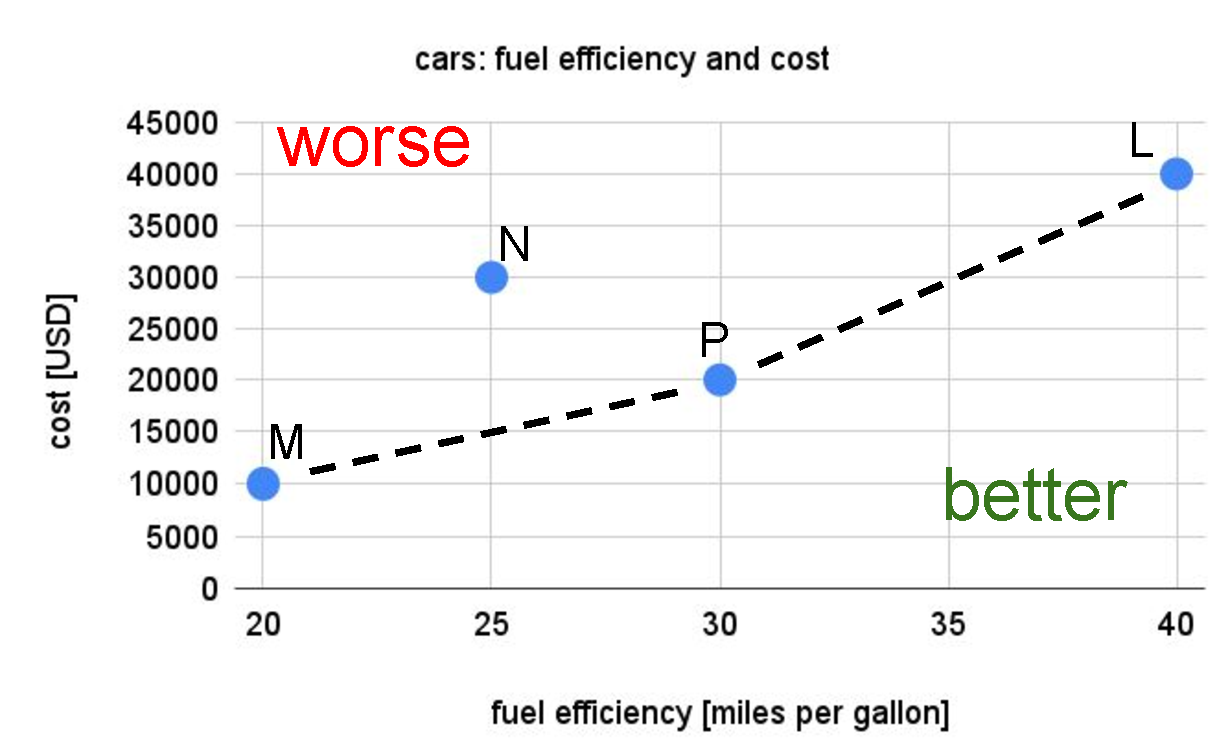
\includegraphics[width=1\textwidth]{images/pareto_frontier_car_options.pdf}
    \caption{Four cars, L, M, N, and P. Goal is to spend less money and get better fuel efficiency. Choices not on the frontier should be avoided, but that doesn't yield a single result.}
    \label{fig:pareto_frontier_cars}
\end{figure}

A common pareto frontier in generic decision making is the trade-off between speed, accuracy, and cost. 

Pareto frontier analysis works well when there are many options relative to the number of variables being optimized for. Does not account for relative importance of different variables.

The assessment does not work as well when there are few choices relative to the number of variables. For example, suppose there are 10 choices of car and I want high fuel efficiency, high cargo capacity, maximum number of passengers, stylish, low cost, low maintenance, good durability, and high resale value. might need to assign weights to each of these factors. 

A typical decision is ill-informed, has diffuse consequences, delayed impact, and does not affect the decision maker. 

Even afterwards a decision can be difficult to evaluate for correctness because there are multiple stakeholders.

In bureaucratic processes there is rarely a formal assessment of options. 
Decisions are rarely recorded. 

Decision making by bureaucrats can be informal or formal, consensus-based or solo. 

Most decisions made by bureaucrats do not have hard deadlines. Instead, there are trade-offs in timing. Sooner is better, but delaying allows for more information gathering for a better informed decision.




Decision makers face options and have the goal of identifying a beneficial outcome (for which stakeholders?). The goal is to reduce uncertainty among options. Two ways to reduce uncertainty: gather more information (takes time), or push the decision down the chain (to people with narrower view). 

If a bureaucrat is going to rely on expert consultation, the decision maker needs to be confident the expert is not of straying outside their area of expertise. For example, I don't rely on a botanist with many published papers to tell me how to change the oil in my car. 

When getting input for a decision, is the expert providing a factual summary, a predictive assessment, or a value judgement? 

There are many ways to gather evidence. 
Role of measurement and modeling. 
Form an opinion, look for evidence to back the outcome.
Instead of measurement, most people rely on history (if they are aware of it), or what is best for their career, or how to accumulate more power, or what someone else says to do.  


\section{History of Bureaucracy}

I'm mostly going to skip history and merely cite other scholarly references


https://en.wikipedia.org/wiki/Bureaucracy
\section{Scope of bureaucracy}
\subsection{Who is a bureaucrat?}

A cashier in a gas station is a bureaucrat. The ``policy'' might simply be ``take money from customer in exchange for items and gas,'' but the subjective application of that policy leaves a lot of room for the cashier to shape the customer's experience. Does the cashier greet the customer when the customer enters the store? Does the cashier look at the customer to acknowledge the customer? Smile? How quickly does the cashier engage the customer? Minor nuances that are left to the cashier in the execution of the store policy means there is room for subjective application of the policy. 

% examples of bureaucrats
A bank teller, a loan officer, and a bank's \href{https://en.wikipedia.org/wiki/Technical_support}{technical support} are all bureaucrats. Each person subjectively enforces policies on behalf of the organization. The directness of financial impact for the person varies among these roles. Of these three roles, the loan officer's interactions with bank customers provides the clearest feedback on profit. The loan officer doesn't act alone though -- the customer's interactions with tellers and the bank's technical systems also matter to the customer's decision. 


This same discretionary application of policy applies to commercial bureaucrats like sandwich makers, car salespeople, oil well drillers, grocery clerks, retail clerks, and plumbers. Public school teachers, state and federal police, military members, tax collectors, and other state workers are government bureaucrats. 


% bureaucracy is not limited to white collard office workers
Factory line workers subjectively apply policies. Enforcement of quality standards is the most obvious area. Pacing of work is a negotiation with management that directly impacts productivity and profits.

Structured environments like sports featuring well defined rules do not eliminate bureaucracy. Teammates use subjective policies on who to work with and how to best leverage their strengths and exploit the opponent's weaknesses. The policies are set in part by the coach. Referees make subjective determinations about rules.

Sometimes bureaucrats do not work directly with customers or citizens or products. Then the bureaucratic process is inflicted on fellow bureaucrats. In this scenario, a bureaucrat is subjectively applying a policy to other bureaucrats. 

Identifying yourself as a bureaucrat matters, both to the employee and to the business. The risk of not self-identifying as a bureaucrat is that you won't grasp how much control you have in implementing and enforcing policy. If you think of yourself as having to blindly follow rules, you will harm the people you are applying the rules to and you will harm the business/institution you are applying the rules for. Adapting policies to circumstances is the value of having judgement capacity. 

In a similar sense from the consumer/citizen perspective, if you don't think you are interacting with a bureaucracy, you won't perceive the opportunity to negotiate.  If you view rules as fixed and inflexible, you will harm your ability to make progress. If a rule was made by a human, then that rule is flexible. Who made the rule? Who enforces the rule? If you can talk to them, could they be convinced to make a modification or an exception?

If you don't think about a bureaucratic framing, you might think the store clerk is enforcing a policy because they don't like you. Assigning personality conflict as the cause might lead to a different conversation with their manager (the person who created the policy). 

If you don't think of yourself as a bureaucrat, you'll behave differently in your job. The paradigm of ``just tell me what to do'' is the default (learned in school) and you won't know how to engage with coworkers/bosses since they are not friends. You will be less likely to understand how to leverage the organization and identify collective wisdom. Thinking from the perspective of a bureaucrat explains why evangelizing within your organization is relevant. 
%You'll see your coworkers as competitors for promotion.

% https://graphthinking.blogspot.com/2020/10/impact-of-self-identifying-as-not.html
If you think of yourself as merely a cog in a machine, you are less likely to notice that you exert influence in the process and you are less likely to recognize the autonomy available to you. 
If you think ``I have a real job (e.g., nurse, cashier, teacher), therefore I'm not a bureaucrat", you are less likely to recognize the subjective power you have in interactions with the public.
If you think, ``I'm at the bottom of my organization's hierarchy, therefore I do not have power", you are less likely to notice the autonomy when it is available.

If you don't think of yourself as part of a bureaucratic process, you'll behave differently in interactions with bureaucrats.  You won't perceive opportunities to negotiate because the processes seem fixed instead of subjective. 
You won't recognize motives and incentives of bureaucrats, so their activities will seem incomprehensible.


 % subsection
\subsection{Number of People in a Bureaucracy}

Although bureaucracy can be present for one person, and bureaucracy is often apparent on teams (e.g., 3 to 20 people), this book focuses on the situation of multiple teams comprising an organization. This might be a few hundred people (above \href{https://en.wikipedia.org/wiki/Dunbar's_number}{Dunbar's number}) up to millions of people. 
Examples of companies that employ more than a million people\footnote{see \href{https://en.wikipedia.org/wiki/List_of_largest_employers}{Wikipedia's list of largest employers}} include Walmart, Amazon, and McDonald's. Size isn't a requirement for bureaucracy. Small companies with a few people incur bureaucracy because of the need for coordination of subjective policies governing shared resources. Non-profit organizations encounter bureaucracy. 
Bureaucracy emerges in small organizations, has patterns that are scale invariant, and is generic across sectors. The complexity of the tasks may be different, but the same scale-independent patterns can emerge because of a common factor: human behavior.

% https://graphthinking.blogspot.com/2017/05/population-sizes-needed-to-support.html
The size of bureaucracy scales with the complexity of the problem. For example, if participants in a society only used hand tools they could make themselves, then there is little need for bureaucracy. Mining and producing small amounts of metal is feasible for an individual, though the relevance of specialization becomes clearer. A society large enough to support the technology of writing (beyond the use of clay tablets) seems to coincide with the bureaucratic need for writing. Getting to technology like the telegraph and radio requires a society that supports complex processes and specialization -- key aspects of bureaucratic systems. While decreasing bureaucracy is certainly feasible, it's not clear how to maintain the current technological sophistication. 


In addition to essential task complexity, the size of bureaucracy depends on accidental factors like how old the bureaucracy is, how big the community being supported is, and how diverse the community is.


 % subsection
\subsection{What does Bureaucracy imply?}
Bureaucracy is neither good nor bad. Bureaucracy is not tied to politics, or any specific institution (corporations, governments, academics). Bureaucracy is not defined to be efficient nor, does it have to be inefficient. Bureaucracy is not restricted to paperwork, or record keeping, or quantification, or gathering metrics. 

Bureaucracy is about delegation of control, communication, decision making, coordination, and processes. Involves negotiation, primarily informal. In that context, wouldn't it be useful to be skilled at bureaucracy?  % section
\subsection{Why does bureaucracy exist? Can't we just do the work?}

Monarchies and dictatorships the rely on a single decider. A simpler model to understand, but difficult to handle all the edge cases for large society. 

Political representatives are an easier to understand concept because it's just one person acting in that behalf of other people.
In contrast emergent behavior of bureaucracy is more difficult to understand. TODO: why not make the entire system out of politicians?

TODO: thought experiment: 
What if everybody in a bureaucracy were the same?
What if everybody in a bureaucracy had a different opinion?


The short answer is that bureaucracy is a response to the complexity of a problem being solved. To see why that is, let's start simple and then increase the complexity. 

The minimal scenario to start from is to imagine a single person working on a single task that does not last long (a few minutes), is relatively easy (cognitively and physically and emotionally), and does not recur. In that situation, building consensus is irrelevant and no process is required. 

Most of what you do occurs outside those limits and thus incurs some concept of \gls{process} (breaking a task into subtasks). Staying with the one-person constraint, a complex task can benefit from being broken into subtasks. Sometimes the order of the subtasks matters, so we need to track the dependencies. A recurring multi-step process with documentation is starting to have features of bureaucracy, but lacks the need for consensus. 

If one person lacks the skills relevant to a multi-step process, they may engage another person to help. The interaction may be informal (anarchy) or formalized in a contract (\href{https://en.wikipedia.org/wiki/Libertarianism}{libertarian}). If the parties working on the task fail to reach consensus, what is the recourse? Options include physical violence, threats, or involving a third party (e.g., a court with lawyers and judges). 


The bureaucrat's identity is subsumed into service for the organization they are part of. At the same time, bureaucracy enables the bureaucrat to amplify their presence by being part of a larger organization. A bureaucrat can accomplish more as part of an organization than by working alone. Sometimes the cost of being part of the organization exceeds the force multiplier of working together. 

% https://graphthinking.blogspot.com/2021/09/why-is-everything-so-hard-in-large.html

What if we completely avoided bureaucracy? That question is better worded by replacing ``bureaucracy" with ``coordination of stakeholders". If you avoid coordination of stakeholders, you either are constrained to only work on tasks that involve one person, or you get is random (uncoordinated) interactions. 

What if we minimized bureaucracy? Again, try replacing ``bureaucracy" in that question with ``coordination of stakeholders". The goal of ``minimizing coordination" probably isn't the real objective. To be more precise, a specific objective might be ``minimize time spent executing the task" (which takes a lot of coordination prior to the task execution) or ``minimize the level of distraction to stakeholders" (chunk the coordination time). Another strategy for minimizing bureaucracy is to reduce the number of stakeholders involved. For a given task complexity, this means having smarter people who have more skills. 

\begin{figure}
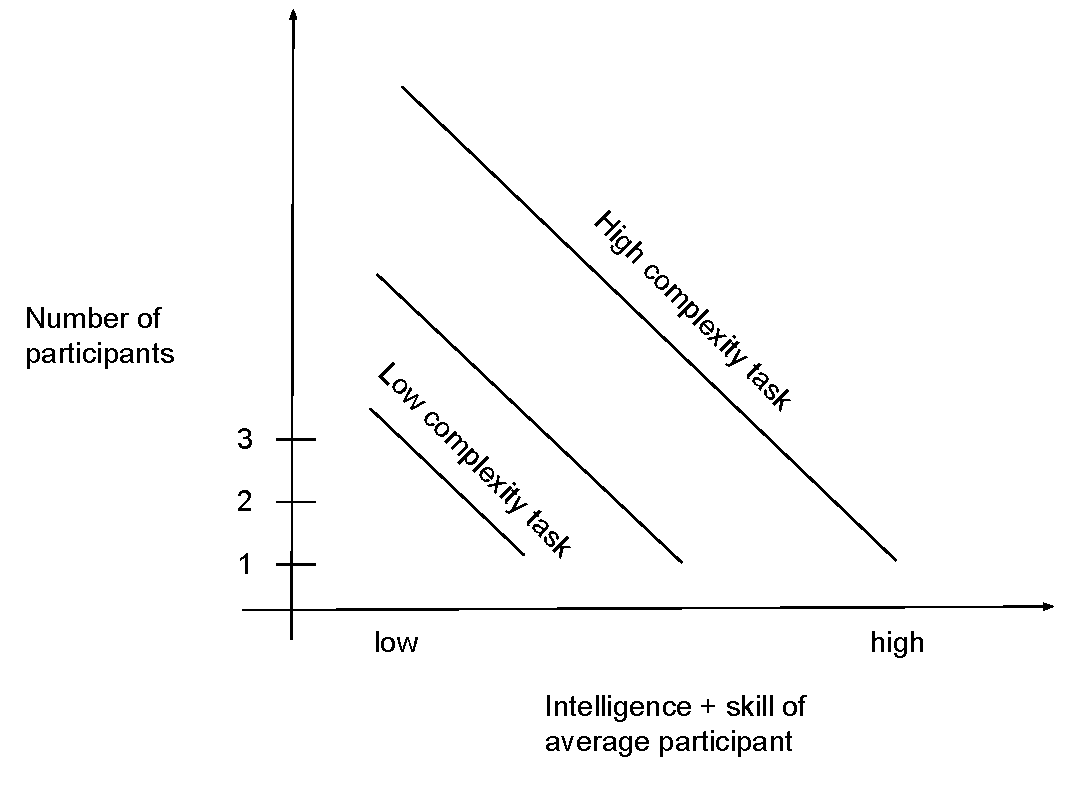
\includegraphics[width=0.8\textwidth]{images/people-per-task-for-skill-level.pdf}
\caption{Three levels of task complexity are shown. As task complexity increases, the size of the team needs to grow. The growth may be less if the team members are brilliant. Those brilliant people cost more and there are fewer of them available.}
\end{figure}
 % section
\subsection{Why is bureaucracy so hard?}

When a person has a positive experience engaging with bureaucracy, positive attribution is made to the people involved. Or ease of a solution makes the bureaucracy less visible and the solution seems obvious. 

When a person has a negative experience with bureaucracy, complaints are about the incompetence of the people involved, or the incomprehensibleness of the system. Don't these bureaucrats know how to do their job? Why isn't the solution obvious? Why does this system not work for me?

many nuances not visible to external perspective
\begin{itemize}
    \item organization politics (personalities, resources, prioritization)
\item lack of unified voice
\item legacy policies to overcome/change/be consistent with
\end{itemize}





\chapter{Bureaucracy throughout life\label{b_throughout_life}}
This chapter provides the view of a person interacting with bureaucracy as a user. 

Personal routines are self-imposed bureaucracy
\section{Avoiding Bureaucracy is Nearly Impossible}

The only situation where bureaucracy might not exist is if you live completely on your own, with no interaction with other people. That means completely disengaging from society. Even then, personal routines are a self-imposed form of bureaucracy, with the roles of policy maker, bureaucrat, and subject collapsed to a single person -- you.

Self-sufficiency and autonomy are attractive alternatives bureaucracy. The way participants in modern society strive for self-sufficiency is by denying their dependence on modern society. That's a relabeling of selfishness which feels better. 

For the rest of us who operate as members of a society, bureaucracy is necessary for our rights. We prove our name by cooperating with other people, and our name helps us claim our citizenship. That's a subjective policy that \glspl{stakeholder} in society agree to. 



The specific way a society is constructed (democratic, authoritarian, dictatorship, anarchy) is irrelevant -- bureaucracy is still present. Even the libertarian view of relying on contract enforcement implies some amount of bureaucracy (e.g., forums for resolving contract disputes like a court system). 


Not all bureaucracy is due to the state, nor is bureaucracy confined to companies. Parenting involves coming up with situation-specific requirements for children, with the organization being the family as mentioned in \S\ref{sec:bureaucracy-early-childhood}. Dress codes for sports teams are arbitrary standards. 
Store clerks are bureaucrats, as are website forum moderators.  Content moderation is the process of (inconsistently) enforcing arbitrary standards. This mindset even permeates individuals as internalized expectations of policy and enforcement when no one else is present. 

Recognizing instances of bureaucracy enables more skillful interaction, whether as a bureaucrat or as a subject. The remainder of this section  illustrates both the view of a person interacting with bureaucracy as a \gls{subject}, and the perspective of bureaucrats working within organizations. 





\section{Beginnings and Endings}
In life there are some standard milestones: birth, education, work, death. Each of those milestones corresponds to engaging bureaucracy. 

Within the employment phase, there are pairs start and end events which may apply: hiring or getting hired; firing, getting fired, or quitting. 


\section{Relationships throughout life}
In the conventional Western progression, relationships include
\begin{itemize}
    \item pre-education childhood: primarily family, possible community members, caretakers
    \item primary education: family, friends, teachers
    \item college, graduate school: friends, teachers, advisors
    \item employment: managers above you, peer employees, people you manage
    \item healthcare
\end{itemize}

\subsection{school vs business}
School (high school, undergraduate, graduate school) is  different from working in a large organization. 


\subsection{undergrad vs graduate}
 education process roles and expectations vary over time

\subsection{military}
Less than 0.5\% of the United States population serves in the military. \footnote{source: \href{https://www.cfr.org/backgrounder/demographics-us-military}{Council on Foreign Relations}}

The military, with rigid hierarchy and defined protocols, is also a distinct experience. 



\chapter{Bureaucracies are made of Humans\label{b_made_of_humans}}
This chapter provides an insider's perspective of working in a bureaucracy. What are all the aspects to consider?
% unordered essays to be clustered later

\subsection{Hiring into a Bureaucracy}

Hiring shapes the culture of an organization and determines what is feasible, both by the skills of those hired and how well new hires integrate with the existing organization. 

Hiring is an expensive process in terms of money, time, emotional investment of candidates, and the burden of reviewing applicants. 
% SO WHAT? What's the consequence?

When hiring into an organization there is a selection bias in the people who join a bureaucracy, and there is a selection bias who stays in bureaucracy. 
% SO WHAT? What's the consequence?



Regardless of the specifics of the job, there are specific attributes that make a candidate more likely to be successful in a bureaucracy. In addition to role-specific skills, hire for \href{https://en.wikipedia.org/wiki/Metacognition}{metacognition}, social skills, and intrinsic motivation.

% https://graphthinking.blogspot.com/2021/04/screening-for-metacognition-in-job.html

% https://graphthinking.blogspot.com/2021/07/screening-for-intellectual-empathy-in.html

% https://graphthinking.blogspot.com/2021/04/questions-to-ask-interviewer-when.html


\section{professional training}
\section{Folk Wisdom}
While most of the entries on
 \href{https://github.com/dwmkerr/hacker-laws}{https://github.com/dwmkerr/hacker-laws}
don't apply to bureaucracy, the list is useful to review. 

% https://www.timsommer.be/famous-laws-of-software-development/

Folk wisdom is an attempt to explain bureaucratic features using a simplistic model.

\subsubsection{Organization chart orientation
\label{org-chart-orientation}}

A common method of describing relations within the bureaucracy is the organization chart (colloquially, the ``org chart"). Normally the CEO is at the top of the chart, middle management is in the middle, and managed employees are at the bottom. See figure~\ref{org_chart_orientation_ceo-at-top} 


An organization's culture is subtly conveyed by artifacts like org charts. 
% What's the point of this section? Is there a consequence, or is this just an observation?
There are emotional connotations to alternative layouts. You can alter expected relations (culture and norms) by playing with orientation of the org chart.
Org chart orientation can be overanalyzed, so this exploration is limited.

The point of thinking about org chart orientation is to frame how you perceive your supervisors, peers, subordinates. Notice that the framing is embedded in the words -- prefixes super (over) and sub (under). 
These concepts inform what you expect from relations.
Do I seek support or direction and guidance from my boss? What do I expect from my boss, peers subordinates? What do I expect to provide them?

%\begin{itemize}
%\item 
%\end{itemize}

The relative orientation of the \href{https://en.wikipedia.org/wiki/Chief_executive_officer}{CEO} to workers sets expectations for relations. 
Options for orientation are the conventional CEO at top
(figure~\ref{org_chart_orientation_ceo-at-top}), 
CEO at the bottom (figure~\ref{org_chart_orientation_ceo-at-bottom}),
CEO on the right (figure~\ref{org_chart_orientation_ceo-leads}),
CEO on the left (figure~\ref{org_chart_orientation_ceo-follows}),
CEO as the center of a star 
(Example: \href{https://en.wikipedia.org/wiki/File:League_of_Nations_Organization.png}{League of Nations diagram})

\begin{figure}
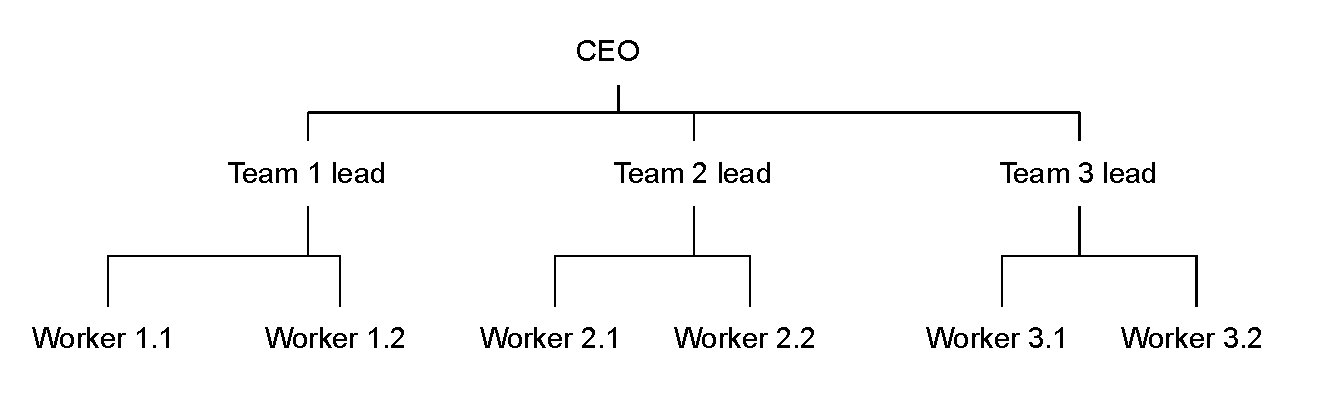
\includegraphics[width=1\textwidth]{images/org-chart-orientation-ceo-at-top.pdf}
\caption{Standard orientation. Role with most responsibility and authority is at top. Left-right ordering is intended to be irrelevant in this view, though left-to-right reading order emphasizes importance.}
\label{org_chart_orientation_ceo-at-top}
\end{figure}

\begin{figure}
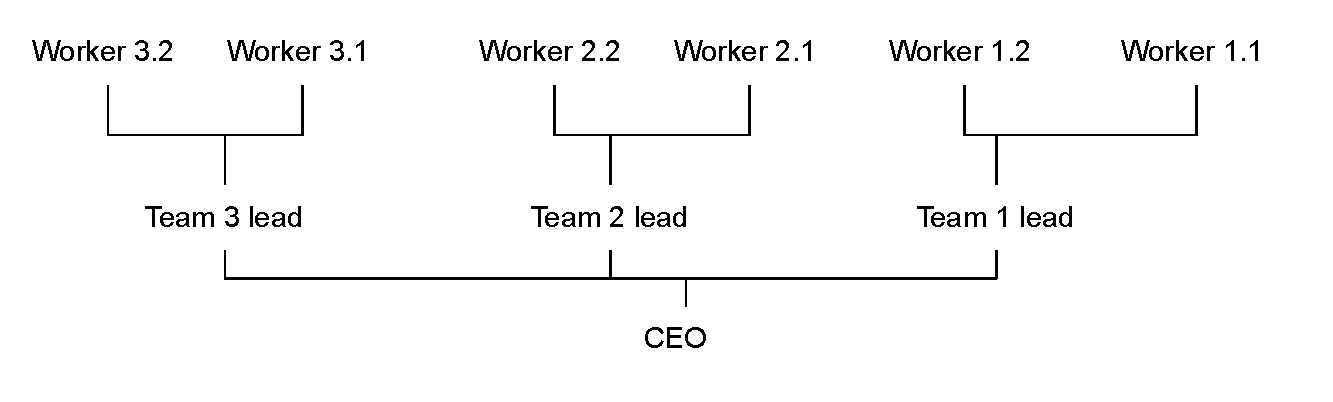
\includegraphics[width=1\textwidth]{images/org-chart-orientation-ceo-at-bottom.pdf}
\caption{Flipping the orientation presents a more realistic view of the CEO's responsibility. The crushing burden of servant leadership is clear. Left-right ordering is intended to be irrelevant in this view.}
\label{org_chart_orientation_ceo-at-bottom}
\end{figure}

\begin{figure}
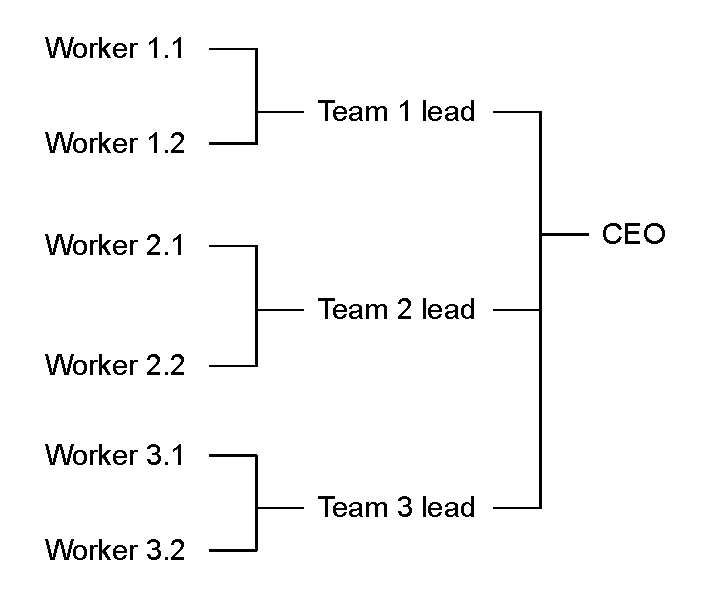
\includegraphics[width=0.8\textwidth]{images/org-chart-orientation-ceo-leads.pdf}
\caption{Conventionally time flows from left (old) to right (new), so in this graph the CEO leads the charge into the unknown. Is the CEO dragging workers forward, or are the workers pushing the CEO? The top-to-bottom ordering can be read as importance. }
\label{org_chart_orientation_ceo-leads}
\end{figure}

\begin{figure}
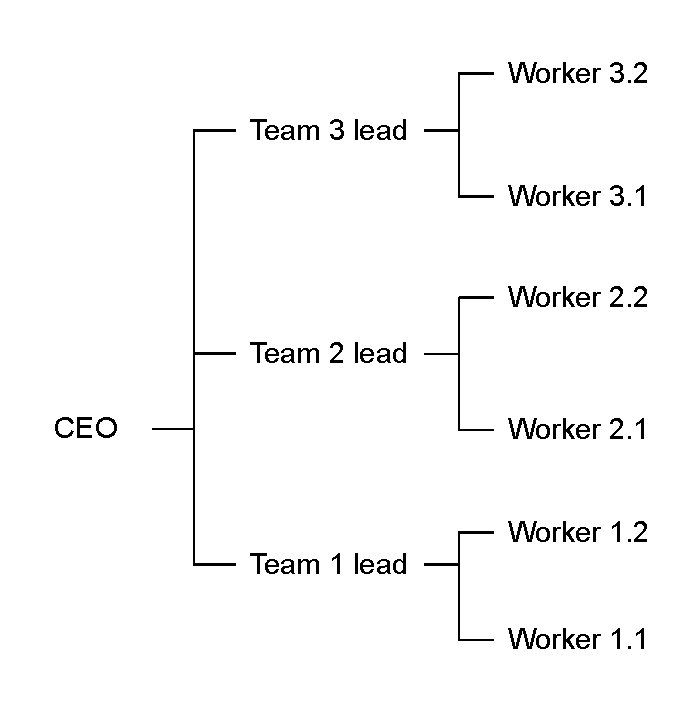
\includegraphics[width=0.8\textwidth]{images/org-chart-orientation-workers-lead.pdf}
\caption{The ``chariot view'' with the CEO in the chariot and the workers out front. Workers are in the future, the CEO is in the past operating on old information. As with figure~\ref{org_chart_orientation_ceo-leads}, top-to-bottom ordering can be read as importance. }
\label{org_chart_orientation_ceo-follows}
\end{figure}



%extension of 
% \href{https://en.wikipedia.org/wiki/Conway\%27s_law}{Conway's law}: seating chart reflects org chart
essential bureaucracy is the minimum necessary to address the complexity of the problem space. This is tricky since the optimization can be with respect to resilience to change, resilence to edge cases, staff turn-over, speed experienced by consumer, financial cost, organization time, organization staffing level.

Undesirable bureaucracy is either accidental or legacy
% https://graphthinking.blogspot.com/2021/02/how-to-have-efficient-bureaucracy.html

In an ideal scenario with no bureaucracy, everyone comes to the same conclusion when presented with the same information. Then the management process of building consensus becomes unnecessary. There is no need to fight over resources (money, staffing) and no need to fight over direction.

While that ideal scenario is not going to happen, it points to how to improve bureaucratic efficiency:
\begin{itemize}
\item each person has the same information. 
\item each person applies the same decision making process consistently
\item every person has the same incentives
\end{itemize}
The reason bureaucracy is inefficient is
\begin{itemize}
\item not everyone has the same information
\item processes are inconsistent
\item incentives vary
\end{itemize}
Also, add the issue that each person's reference experiences are unique. As a consequence, decision making is subjective. 

Can any action be taken to improve bureaucratic efficiency? Yes!
\begin{itemize}
\item you can share information with other stakeholders
\item you can seek information from other stakeholders
\item you can strive for and demonstrate transparency
\item apply consistent processes 
\item hold others (and yourself) accountable 
\item account for varying incentives and reference experiences
\end{itemize}

\subsection{Motivation of Bureaucrats}

To understand the bureaucrats you work with, appreciating their diverse motives is instructive. If you expect everyone to have the same motives as you, then you will be surprised by the friction. 

Motivations of participants are rarely ``how can I make the company more successful" or even ``how can I sell/produce more product"? Usually motivation is based on personal success in various manifestations, which leads to emergent phenomena which appears confounding to observers outside the bureaucracy. 


% see https://en.wikipedia.org/wiki/Social_influence

Each bureaucrat has a motive, even the bureaucrats who do nothing. 
% https://graphthinking.blogspot.com/2020/02/there-is-no-idle-status-for-paid.html
In an organization where you are a paid bureaucrat, you are either actively working for improvement of the organization, or your existence is parasitic to the organization. There is no ``idle" status for paid employees in an organization with limited resources.

Not too efficient such that I eliminate the need for my job, and not so inefficient that the organization fails and I lose my job. Increasing the efficiency of bureaucracy is good for the organization and the outcomes, but can be harmful to the bureaucrat's career.

Career stability within an organization is a benefit, and it can be leveraged to take more risk. However, it typically manifests as inaction by an employee. There's no harm to the employee in not taking action. If an employee doesn't do anything, nothing bad will happen to that employee. Career stability decreases extrinsic motivation.



Example motivations for bureaucrats: stability, money, travel, problem solving, like being associated with org, logistical convenience (``the office is near where I lived.'')


% https://graphthinking.blogspot.com/2021/04/laffer-curve-and-minimum-viable.html

The Laffer curve is a claim in economics that there is a relation between government tax rates and the revenue from taxes collected. The relation, based on Rolle's theorem, says that between a tax rate of 0% and 100%, there must be some amount of tax that corresponds to the maximum of revenue. 

While the mathematical statement may be provable, the use in economics seems hand-wavy. In this post, I'll extend that hand-waviness to a different domain: bureaucratic processes in organizations. The relation to the Laffer curve is that bureaucratic processes a tax on productivity. 
\section{Bureaucratic Fallacies\label{sec:fallacies}}

There are perspectives that are \gls{thought terminating}. Identifying these enables you to understand both why they are attractive and how they are incomplete.

See also unavoidable hazards in \S~\ref{sec:unavoidable_hazards}.

\ \\

\textit{Bureaucratic fallacy}: \textbf{Bureaucracy is bad}. \\
\textit{Why this feels true}: when a person subjected to bureaucracy has a negative experience, the easiest attribution is to the least-understood aspect -- the bureaucracy.\\
\textit{What this is missing}: \Gls{bureaucracy} is neither good nor bad. 

\ \\

\textit{Bureaucratic fallacy}: \textbf{There is no point in planning ahead since everything (staffing, funding, purpose, scope) is always changing.}\\
\textit{Why this feels true}: Change can feel disorienting, especially when it is unexpected. \\
\textit{What this is missing}: Preparing for change and thinking ahead about contingencies enables effective use of resources. Have a vision and work towards it while accounting for change. 


\ \\

\textit{Bureaucratic fallacy}: \textbf{Bureaucracy is an aberration, a mistake, due to poor planning or incompetent participants}. \\
\textit{Why this feels true}: TODO\\
\textit{What this is missing}: TODO

\ \\

\textit{Bureaucratic fallacy}: \textbf{Bureaucracy is inefficient}. \\
\textit{Why this feels true}: Expressed by both subjects and bureaucrats who observe seemingly wasteful processes.\\
\textit{What this is missing}: If bureaucracy were truly inefficient (not allocating resources in the most efficient way), then it would be replaced by a more efficient approach. The key is to ask, ``efficient with respect to what metric?'' The metric of money, time, number of people, stability, robustness to perturbation.  Second, what would motivate improved efficiency? Without incentives, change is less likely. 

\ \\

\textit{Bureaucratic fallacy}: \textbf{Bureaucracy is due to malfeasance.}\\
The specific number of malicious bureaucrats ranges from ``all of the participants'' to ``just enough to be problematic.'' \\
\textit{Why this feels true}: There are bad actors. 
\textit{What this is missing}: Bureaucracy is unavoidable, and most of the participants are earnestly trying to help or are not making a positive contribution. Processes within bureaucracy are used to deal with malicious bureaucrats, like isolation or promotion. 

\ \\

\textit{Bureaucratic fallacy}: \textbf{Bureaucracy is a sign of decay from within the org.} \\
\textit{Why this feels true}: TODO\\
\textit{What this is missing}: Bureaucracy is unavoidable emergence in any/every organization.

\ \\

\textit{Bureaucratic Fallacy}: \textbf{If this request can't be expedited, it must not be important}.  \\
\textit{Why this feels true}: Other people would demonstrate they care about what I am working on by prioritizing things I am dependent on.
\textit{What this is missing}: When everything gets prioritized, that's the same as nothing getting priority.

\ \\

\textit{Bureaucratic Fallacy}: \textbf{Duration of a task is how long it would take one person to accomplish}.  \\
\textit{Why this feels true}: TODO\\
\textit{What this is missing}: Fails to account for the overhead of interaction and delays due to asynchronous engagement.


\ \\

% https://graphthinking.blogspot.com/2019/08/two-misleading-simplifications-when.html
\textit{Bureaucratic Fallacy}: \textbf{Consider the average or majority (to the exclusion of outliers)}. \\
Why this simplification is misleading: For sufficiently large ensembles, the outliers alter the outcome. The larger the ensemble, the more significant the role of the outlier minority.

\ \\

\textit{Bureaucratic Fallacy}: \textbf{people learn from their mistakes}. \\
\textit{Why this feels true}: TODO\\
\textit{What this is missing}: Requires a low latency feedback loop and incentive to change.

\ \\

\textit{Bureaucratic Fallacy}: \textbf{processes are serial}.\\
\textit{Why this feels true}: TODO \\
\textit{What this is missing}: TODO


\ \\

\textit{Bureaucratic Fallacy}: \textbf{Hard work creates results}.\\
\textit{Why this feels true}: TODO\\
\textit{What this is missing}: TODO


\ \\

\textit{Bureaucratic Fallacy}: \textbf{Motivations for bureaucrats are categorized as individualistic, tribal, organizational, societal, or humanity}.\\
\textit{Why this feels true}: TODO\\
\textit{What this is missing}: TODO


\ \\

\textit{Bureaucratic Fallacy}: 
\textbf{you cannot pay a little and get a lot}; see \href{https://en.wikipedia.org/wiki/Common_law_of_business_balance}{Common law of business balance}. \\
\textit{Why this feels true}: TODO\\
\textit{What this is missing}: This doesn't allow for creative solutions and ignores \href{https://en.wikipedia.org/wiki/Nudge_theory}{nudge theory} from behavioral economics. 


\section{Building, Managing, and Spending Reputation\label{sec:reputation}}

% distinct from
%Social Capital https://en.wikipedia.org/wiki/Social_capital
%Political Capital https://en.wikipedia.org/wiki/Political_capital


%How does an individual create and accumulate political capital? What does political capital mean with respect to teams?

This section is about actions you can take to create a reputation and how to spend political capital. 

\subsection*{Relevance of Reputation in a Bureaucracy}

As a bureaucrat you may want to be all things to all people. Since that is not feasible, you have to limit your scope and therefore disappoint some people. This same dynamic of a limited scope applies to the team you are on, and again to the organization the team is part of.

The good news is that you have influence over how others perceive your limitations. Creative negotiation with other bureaucrats, other teams, and other organizations shape their perception of your value. 

\subsection*{Definition of Reputation}

Your reputation as a bureaucrat is what other people expect from you. Reputation is perception. What does that person think of you? Your team? Your organization? 
Reputation is set whenever and where ever you are observed, or artifacts are associated with you. 
What you wear matters, when you show up impacts your image, how your written communication is read alters perceptions, and people are informed by your body posture in meetings. 

\subsection*{Reputation, Brand, Image}

There are multiple phrases that all refer to the same concept of being perceived and the associated expectations. Individuals create (or get) a reputation; organizations have brands. A team of bureaucrats can have a reputation. 

\subsection*{Your Reputation matters}

Your personal reputation within the organization dramatically impacts your effectiveness. People will let you do things (or prevent you from doing things) based on their expectations about you. 

Your reputation matters impacts your influence. Whether other people turn to you for input depends on what they expect from you. How other people perceive you impacts what you can accomplish and when people seek out your help or input.

\subsection*{You can Manage your Reputation}

Managing reputation means acknowledging that your interaction with others is partially performative. This may feel disappointing if you want to be judged solely on your productivity or knowledge. 

Your success is limited if you focus exclusively on doing the work, and your success is limited if you focus exclusively on the performative aspects. 
Neglecting to manage your reputation means you lose input to the stories others tell about you. Active management of your reputation requires engaging people and generating evidence. 

Your reputation is dynamically changing based on your activities and communication. Your communication matters, and the stories other people tell about you matter.

\subsection*{Techniques for Building Reputational Capital}

Ideally your reputation would be a function of your technical skill, your ability to collaborate with other people, the strength of your network, and your creativity. None of those matters if the person you're engaging with doesn't know those things. 
You build reputation by doing things that are useful and visible to other people. This positive association is what you are creating.

Because the definition of reputation is about expectations other people have about you, what you choose to work on matters. How you work on your tasks (creativity, enthusiasm, dedication), the artifacts produced, and your ability to communicate all shape your reputation. 

When building reputation, you can work on multiple small wins or take larger risk on bigger bets. The bigger bets provide faster leverage of reputational capital as you have demonstrated your worthiness and skill. 

The same concepts apply to teams of bureaucrats and bureaucratic organizations. Just as individuals compete for resources, teams compete for budget, staffing, and glory. How the team's budget and staffing are spent impact reputation. 

A specific technique for building a good reputation is to give credit to others (section~\ref{sec:credit-others}).
\marginpar{[Tag] Actionable Advice}
This may seem counter-intuitive if you are focused on the apparent assignment of credit. What actually matters is that other people observe you (whether directly or indirectly) giving credit. 

Similarly, another technique for building good reputation is offering to take blame (section~\ref{sec:take-blame}).
\marginpar{[Tag] Actionable Advice}
Again, this can seem counter-intuitive since being blamed doesn't sound good. The value is in proclaiming your willingness to be blamed such that other people observe your offer. 

\subsection*{Using Good News (or Early News) to build Influence}

Rather than tell good news directly to a top-level decision maker, first inform the person who influences the decision maker.
\marginpar{[Tag] Actionable Advice}
I tell the influencer the information does not need to be credited to me.

The benefits of this approach include
\begin{itemize}
    \item Improves the influencer's reputation with the decision maker.
    \item The influencer has the chance to contextualize the information for the decision maker.
    \item The influencer has the option to leverage the information in ways I would not have.
    \item My reputation with the influencer is enhanced.
    \item I reaffirmed the influencer's role and status.
    \item Influencers are easier to access.
\end{itemize}

\subsection*{How to Spend Reputation}

Based on your reputation (what the other person expects), what trust does that person have?  You can then use that trust to do things that might not otherwise be feasible. You can spend reputation to bend the rules. 

Reputation is not the only thing you as a bureaucrat can spend. Other examples include your time (up to you entire career), your ability to be a member in the team or organization, your self-respect, and your ability to be promoted or receive bonuses. At the level of the team and the organization, additional aspects to spend are the budget and the staff. Each of these (reputation, time, membership, budget, staffing) are potential investments. 
%Confusingly, the investments are not independent. 

There are things I'm not willing to spend: my integrity and my health (physical, mental, emotional).


Whenever you are engaging within your team, you are either actively spending or building your reputation within the team.
Whenever you are engaging with people from outside your team, you are either actively spending or building your team's reputation.
Because of that, spending reputation means taking risk that involve other people.

\ \\

Examples of spending reputation and not getting a return on the investment:
\begin{itemize}
    \item Ask for a favors and provide no value.
    \item Explorer options that other people don't see as worthwhile and then there's no payoff.
    \item Produce nothing of value to the organization or other people.
    \item Talk with people outside your team and misrepresent the efforts of your team.
    \item Speaking honestly about the faults of your own team to people outside your team.
\end{itemize}




%Internal-to-the-org there is cultural norms. 
% https://graphthinking.blogspot.com/2021/01/why-active-shaping-of-culture-is.html


% https://graphthinking.blogspot.com/2018/05/my-evolving-view-on-role-of-my.html


% the following article is useless
% https://www.indeed.com/career-advice/career-development/build-a-reputation
% since it reduces to "be a good person"


% https://graphthinking.blogspot.com/2021/09/notes-from-class-on-being-politically.html



\section{product deployment}

\subsection{external to the org}
\subsection{internal to the org}
\subsection{Actual time spent working}

% What's the point of this? Is there a consequence for the reader?

In a bureaucracy the actual time spent working is less than the number of hours you get paid for. Breaks during work, vacation from work, holidays, sick leave. 

% https://rescuetime.wpengine.com/work-life-balance-study-2019/

\begin{figure}
    \centering
    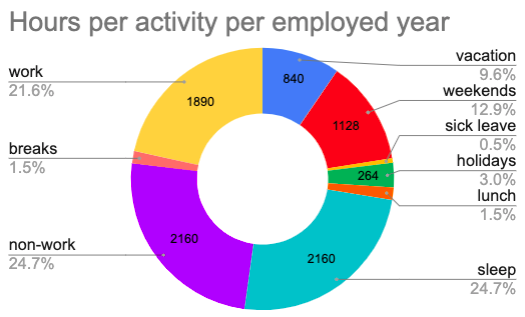
\includegraphics[width=0.8\textwidth]{images/hours_per_activity_per_employed_year}
    \caption{Hours of ``work'' per year when accounting for the rest of life. Assumes 5 weeks of vacation, 2 days of sick leave, and 11 holidays.}
    % footnotes in caption is not recommended; see https://texfaq.org/FAQ-ftncapt
    % however it can be done; see https://stackoverflow.com/questions/67621322/footnote-in-caption-of-figure-on-latex
    \label{fig:hours_per_year}
\end{figure}

Fig~\ref{fig:hours_per_year}
\footnote{\href{https://docs.google.com/spreadsheets/d/1ZaOZZXWkEzX4fFltUdlR4A6ENrAXnkzTW4YrjA4tDO8/edit?usp=sharing}{source for calculations}}
% https://graphthinking.blogspot.com/2021/07/patterns-anti-patterns-in-bureaucracy.html

% intra- and inter- team dynamics

\section{Teams as a subdivsion of an Organization}

In the context of altering teams, there are a few major levers available: create new team, merge teams, dissolve a team. 

For a given set of teams, the lateral interactions are competitive or cooperative. Coordination is required (or conflict will occur) for money, staffing, and resources. Examples of resources include access to or control of data, computer equipment, hardware, floor space, prestige, products (output)
\section{Communication within a Bureaucracy}
% https://graphthinking.blogspot.com/2020/05/invisible-bureaucracy.html

\subsection{Social and Bureaucratic interactions}

Interactions with other people in an organization are either social interaction or bureaucratic interaction. 

As examples of each of these,
\begin{itemize}
\item Social interaction example: "Did you see the game on TV last night? Our team really did well, right? I thought about getting tickets for the game but they were sold out."
\item Bureaucratic interaction example: "You'll need to get approval from Sue before presenting your idea to the board for their review. Then talk with Russ and get his thoughts."
\end{itemize}
Both social and bureaucratic interactions are vital to cohesion in an organization of people. 


Bureaucratic interaction can be broken into two subcategories: \gls{visible bureaucracy} (procedures and processes are written down and can be discovered by stakeholders)  and \gls{invisible bureaucracy} (procedures and processes are known to some stakeholders and are conveyed verbally to some of the other stakeholders).

Invisible bureaucracy is akin to invisible domestic or relation work outside the professional environment. The work associated with emotional cohesion, logistics, planning, scheduling, and communicating is hard to quantify so it does not get counted.

To make invisible work and invisible bureaucracy visible, document the work.


The relevance of this jargon is to break down the components of an organization's "culture" experienced by participants. The ratio of social/visible bureaucracy/invisible bureaucracy is a characterization of the culture. There are norms associated with each of these three categories. % subsection
\subsection{Communication Tips}

The role of verbal communication is critical for bureaucrats. 
There is a lot of advice on effective communication (enunciate, speak loud enough to be heard, be humble, be curious), so the advice below is highlighted because of prevalence in bureaucratic organizations. 
The following is generic to interactions outside of bureaucracy. 

For general writing tips, see Strunk's and White's Elements of Style and other resources \footnote{\href{https://www.youtube.com/watch?v=vtIzMaLkCaM}{LEADERSHIP LAB: The Craft of Writing Effectively} and \href{https://www.youtube.com/watch?v=aFwVf5a3pZM}{LEADERSHIP LAB: Writing Beyond the Academy}}.

\subsubsection{Tip: Not all interaction challenges are communication problems.}
Sometimes an inability to discuss ideas is not a communication problem but a psychological deficit of personality. Distinguishing ``I'm an ineffective communicator'' from ``the person I'm talking with doesn't communicate effectively'' from ``that person has a diagnosed psychological reason they are unable to communicate'' is tough for those of us who are not psychologists or psychiatrists. 

%how to measure effectiveness: The waste or inefficiency in a bureaucracy is a measure of the lack of coordination or inconsistent decision making among the members

\subsubsection{Tip: Avoid relying on stereotypes.}
Within an organization different teams may build up reputations for certain behaviors, or there may be significant events that the team is associated with. 
When interacting with members of a team that has a reputation, avoid relying on that stereotype or event as an opening for discussion. 
You're speaking to an individual, so address that person's behavior.



\subsubsection{Tip: Avoid questions that have a binary response\label{sec:yes_no_questions}.}

Responding to a request with ``no'' is advantageous for the person replying to the question. There is less work required, less risk of failure, and better continuity. As an example of a poorly framed question, I could ask, ``Can I have a copy of the data you're using?'' The person I'm asking is less disrupted if they refuse to share. 

A more constructive phrasing is ``I need information on X to work on Y, and I think you have information about X. How can you help me get information on X?'' By clarifying my intent, I allow the person with the data to provide options I may not have considered.

Similarly, when I'm being asked for information, I try to learn the person's intent motivating the question. Sometimes the requester doesn't actually know what to ask for. Instead of ``no'' I try to figure out how to enable the person to be successful. 

\subsubsection{Tip: Leverage the other person's experience while focusing on your own\label{sec:advice}}

Advice without context is less effective.\\
\textit{Bad}: ``Here is what I think you should do in that situation.''\\
\textit{Better}: ``Here is what I did in that situation.''

People usually find talking about themselves an easy topic if you are curious about their experiences. 
If you can learn the other person's background and history and motivations, you can weave that into the advice you provide. 
Tailoring your message increases the likelihood of implementation. 

\subsubsection{Tip: Avoid Platitudes\label{sec:platitudes}.}
% https://graphthinking.blogspot.com/2017/10/why-platitudes-are-used.html
\href{https://en.wikipedia.org/wiki/Platitude}{Platitudes} are \gls{thought terminating}; the statement feels true and is resistant to debate. Platitudes capture a feeling with sufficient accuracy, but with imprecise language. As a result, there's no specific action.

Because platitudes result in a conclusion, the conversation participants may feel more bonded. However, that bond is shallow.

Example platitudes to avoid:
% https://graphthinking.blogspot.com/2017/02/phrases-which-serve-as-thinking-stoppers.html
% https://graphthinking.blogspot.com/2017/10/a-list-of-platitudes.html
\begin{itemize}
    \item pick your battles
    \item Some things you can't explain
    \item Your time will come.
    \item You can be anything that you want to be
    \item I just want to get through this day
    \item It is what it is
    \item I'm just one person
    \item That's that
    \item Life's not perfect
    \item Life's not fair
    \item There's only so much you can do about it
    \item What is meant to be will be
    \item It is God's will
    \item It's part of God's plan
\end{itemize}

If your goal is to understand a concept or issue deeply, you need to use precise language.

\subsubsection{Tip: Strive to use Precise Language}

Imprecise language causes miscommunication. Intent is unclear, as is expected consequence.

If you have a specific definition for a word central to the topic of interest, ask your new collaborator for their definition. Do not expect others to share your definition even when there are established norms for the topic. 

Instead of asking a collaborator, ``Are you taking action on this topic?'' ask ``What actions are you taking on this topic?''

If someone claims, ``We plan to get to that action,'' ask for a timeline. A deadline can be for an artifact or a re-evaluation of the topic.

In the short-term imprecise language takes less work to create and can take less time to convey. 

The importance of precise language is proportional to the potential consequences of action/inaction/wrong action.
Precision also should be proportional to the complexity of the topic being discussed. 

\subsubsection{Tip: Word is bond\label{sec:word-is-bond}}

Your communication (verbal, written) is your reputation. People rely on what you tell them even if there isn't legal recourse. Reliance on your word is why precision matters. 

Frustration and disappointment follow when you don't uphold your word, or others misinterpret your imprecise language, or you are misunderstood.

Communication implies responsibility for the content.  There is a corresponding accountability in the relationship between speaker and listener (or writer and reader).

\subsubsection{Tip: Take care near the boundaries of knowledge}

Trying to find someone else's extent of knowledge is tricky -- they don't want to appear stupid. They may interpret the exploration at a trap. ``I don't know'' can be an embarrassing statement to make, even if you don't share their embarrassment. 

Knowing the limitations of your own knowledge and disclosing those boundaries to others is critical. Distinguish what you know from speculation about things you don't. 

\subsubsection{Tip: Listen all the way to the last word of the speaker}

Formulating a response to the first part of an idea or a sentence is tempting. Waiting for the speaker to finish before thinking of how to response is courteous. Waiting creates a pause which makes you seem more thoughtful. 

This is complicated by the speakers who include long pauses for contemplation and then resume. 

\subsubsection{Tip: Eliminate speaking over other people.\label{sec:crosstalk}}
% https://graphthinking.blogspot.com/2017/10/crosstalk.html

Crosstalk occurs two people who are communicating verbally experience interference from another audible conversation. That can occur because a third person is talking at one of the original two participants, or when four or more people are holding two separate conversations concurrently. 

Crosstalk in a bureaucracy is motivated by
limited time available to communicate. A meeting participant may feel inspired by something someone else said and want to interject. 
%Typically manifests as popcorn style stories based on experience. 
%Intended as wisdom for self-validation by others in our community. 
Crosstalk can indicate engagement and enthusiasm, or it can be due to the speaker wanting to dominate the topic through interruption. The likelihood of crosstalk is dependent on the level of aggressiveness of participants.
In either case (enthusiasm or power-seeking), the original speakers are disrespected. The original speaker may feel annoyed at being interrupted.



%Crosstalk has four roles and a minimum of two people participating: the discussion facilitator, the original speaker, the interrupter, and other meeting participants. 
%During crosstalk, the discussion facilitator loses control of the interaction to the interrupter.  
The audience is frustrated by the lack of clarity of where to focus. This distraction causes participants to lose of focus and productivity of the interaction decreases.

Bystander intervention for out-of-control meeting: raise your hand. \marginpar{[Tag] Actionable Advice} This non-verbally reverts focus back to the discussion facilitator. 

\subsubsection{Tip: Account for Warnock's dilemma}
% https://graphthinking.blogspot.com/2018/09/dealing-with-warnocks-dilemma-in.html
\href{https://en.wikipedia.org/wiki/Warnock\%27s_dilemma}{Warnock's dilemma}
is the common experience of figuring out how to interpret not getting feedback. This is especially vital in meetings where the speaker or facilitator needs to gauge participant comprehension of delivered content. Simply asking ``Does anyone not understand what I just described?" is likely to get no response from attendees because individuals want to avoid looking stupid.

\ \\
\textit{Technique}: Pick an individual to provide a recap.\\
\textit{Technique}: Survey the audience using multiple choice to gauge understanding.\marginpar{[Tag] Actionable Advice}

\subsubsection{Tip: Seek action with a deadline}

% https://graphthinking.blogspot.com/2017/11/collected-wisdom.html
When asking someone for help or input, specify a deadline for their response. \marginpar{[Tag] Actionable Advice}This helps the person prioritize their tasks.

\subsubsection{Tip: Identify the cause of miscommunication}

% https://graphthinking.blogspot.com/2019/06/miscommunication-versus-inability-to.html
\begin{itemize}
    \item miscommunication the cause is often due to definitions of words used or differences in context. In this situation, additional time spent communicating and taking different approaches is sufficient to remedy the issue.
\item A speaker may be inarticulate. If the speaker is unable to coherently convey their internal experience to a listener, then the communication failure is of a distinct category. No amount of additional communication will lead to improved understanding on the part of the listener.
\item A speaker simply has nothing to say about a subject. Regardless of whether they are capable of articulating a concept, they may be unable to relate to the topic. Often a person in this situation still wants to participate, but they are unable to meaningfully contribute. 
\end{itemize}
% https://graphthinking.blogspot.com/2019/05/identifying-empty-talk.html
Empty talk is the use of words that are ill-defined, emotionally resonant, inactionable, and impersonal.

\subsubsection{Tip: ask-tell-ask}

Collaborating with fellow bureaucrats who have expertise in areas you do not requires extra work. There may be differences in the words used to describe certain situations, more precision in wording that you're used to, or thinking about situations in ways you are not familiar with. In that context, to bridge the differences you can ask, tell, ask\footnote{\href{https://cepc.ucsf.edu/sites/cepc.ucsf.edu/files/Curriculum_sample_14-0602.pdf}{``The 10 Building Blocks of Primary Care: `Ask Tell Ask' Sample Curriculum''} and \href{https://www.the-hospitalist.org/hospitalist/article/125126/qi-initiatives/ask-tell-ask-simple-technique-can-help-hospitalists}{Ask-Tell-Ask: Simple Technique}}. 

The first step is asking what the other person's perspective is on the topic. This helps establish the appropriate level of nuance is and can tell you how that person frames the issue. The second step is to tell the person what you want to say. The ``tell'' step should leverage what you learned from the first ``ask'' step. Use phrasing that is consistent with what you just learned from the other person. The third step is to ask the person what they heard from you. If they are unable to tell you, you may need to refine your delivery. To improve the likelihood of success keep the content in the second step short. 

The ask-tell-ask technique can be used iteratively in the same conversation, especially in discussion complex topics with a new collaborator. \marginpar{[Tag] Actionable Advice}Using ask-tell-ask takes long than just telling but increases the effectiveness of the communication. You also get to learn more about the other person's perspective. 


\subsubsection{Tip: Initial responsiveness and status updates}
In a bureaucracy requiring approval, or soliciting input, sometimes waiting can provide value to the person doing the waiting. The request may be overcome by events, or the person asking may remind which indicates priority.

\subsubsection{Tip: Make deadlines explicit}

Typically requests have two deadlines. The first deadline is when a response is sought. The second deadline is when a response is no longer useful.  

As an example, suppose I am inviting people to a meeting. I send the invitation 5 days prior to the meeting and I want to know who is able to attend by 3 days before the meeting. The second deadline is the time of the meeting. Replies after that second deadline do not help me understand who is going to attend. 

\subsubsection{Tip: Read each email/memo/report to determine the purpose }
% https://graphthinking.blogspot.com/2021/03/read-each-email-to-determine-purpose.html

\textit{Problematic behavior}: scan the text of a message, see if there is immediate action or response needed. If no action or response is needed, go to the next email. \\
 That does not work for emails that contain logistics associated with future events. 

Instead, consider possible intentions of the person writing the email. 

\textbf{Decision needed}. Typically includes context. \\
\textit{Action}: if the team maintains a decision log, update that.
Response is selection of a choice.

Tip: Instead of asking for a decision, ask for if the person is opposed.

Tip: instead of asking for a decision, ask for the go-ahead. This framing biases the respondent towards action (specifically approval) rather than thinking. 

\textbf{Situational awareness}.\\
\textit{Action}: Expected default is no action, but interject if there's an issue.


\textbf{Action or Tasking}.\\
\textit{Action}: Do something within some deadline

\textbf{Approval sought}.\\
\textit{Action}: Confirm or deny

\textbf{Feedback sought}.\\
\textit{Action}: Assessment of proposal


\textbf{Meeting logistics}. Can be an announcement (widely available), registration (limited attendance), or invitation (specific to you). Attendance is optional or require. \\
\textit{Action}: Create or update a calendar event
Response should restate the logistics (time/date/location/purpose) to confirm. 

\textbf{Brainstorming}\\
May provoke a response for building on an idea.
``For your situational awareness, no action needed." Notification of activity by someone else. Or change in plans. 
If needed, a correction to the described direction might trigger a response or even a meeting.

\textbf{Reference} e.g. describing a process or business workflow. Or a citation.\\
\textit{Action}: Copy process documentation to wiki. Copy citation to bibliography.
Acknowledgement response thanking the sender for the update/clarification.

\textbf{Setting a formal policy or issuing an informal edict}\\
\textit{Action}: move the policy/edict documentation to Confluence or Wiki
Acknowledgement response needed only if the edit is aimed at just me or the group I am leading

\textbf{Question}\\
If this is a recurring question, move to a ``Frequently Asked Questions" page on Confluence or Wiki.
Response needed that provides answer or seeks clarification.


Here I'm using ``action" to refer to activities outside the email channel. 

If I read email to figure out the purpose of the email, that will help me determine what action and response are relevant. 

Whether I am the only recipient or on of many receivers can change the intent of the email, and whether I'm in the ``to" or ``cc" field matters. Unfortunately, ``to" versus ``cc" are not reliable indicators since email senders do not reliably conform to the expected use. 



%This categorization of text within emails is a useful natural language processing challenge for machine learning. Currently a few email providers already do some of this with identifying meeting logistics, providing reminders to follow-up, and providing reply snippets. A browser plug-in that differentiates the various purposes of text could help readers determine relevant actions and responses. 

An email sent to multiple recipients may have different purposes for different readers. The reader's role or knowledge may factor into how they interpret the content. The inclusion or exclusion of recipients alters how the content is understood. 

\subsubsection{Tip: Don't seek attribution for contributions; credit others\label{sec:credit-others}}

Give credit to others for good ideas and beneficial actions. Either they accept credit and you are seen as a contributor to their success, or they push back and you look generous. Credit is not a \href{https://en.wikipedia.org/wiki/Zero-sum_game}{zero sum game}.

\subsubsection{Tip: Offer to take blame\label{sec:take-blame}}

Before an action commences, tell collaborators that you are willing to accept blame if something goes wrong. This alleviates their fear of risks.

\subsubsection{Tip: Survey stakeholders}
% https://graphthinking.blogspot.com/2016/01/how-to-solve-and-not-solve-problems.html

Suppose you are a \href{http://www.peacecorps.gov/}{Peace Corps} worker in Africa. You show up and the village doesn't have easy access to clean water. Villagers walk a long ways in dangerous areas for dirty, unsafe water. This is a very obvious problem and all the villagers agree that they don't have good water and that this problem should be fixed.

Implementing the solution would take about a week - get the equipment to the village, drill a well, build a pump.

You could take additional time and involve the villagers in this project. They could participate in getting the equipment, which should lead to a sense of ownership.
But then when the equipment shows up, they don't take action to drill the well. If the well is drilled, it soon falls into disrepair and the villagers are back to doing things they way they used to. What happened?

The villagers don't see access to clean water as the most significant issue. You came in and imposed your view of what the problem is and how to fix it. When you impose your view of what the problem is, the solution won't be adopted by villagers because they don't prioritize it.
It is better to survey the community to see how they operate. What do they think the problems are?
Both leadership and the community members need to provide priorities.

This issue is exacerbated if you come to the village as a representative of a company providing wells. You are biased when you ask, ``Do you have any problems?"

Of course the villagers have water problems which could be fixed with better wells. However, when you get into the details of placing or improving a well, they lose interest. What the community really wants is free installation, zero maintenance, easy to use, and no operational costs. That would improve their life.

When you say there's cost (both initial investment of capital and then operations/maintenance) and a learning curve associated with the solution, then the user's interest wanes -- you are presenting another cost/benefit ratio for them to evaluate. Then they ask ``Can we get by without the well?" Yes, they don't need the well -- they've survived without it.

Novel solutions (in this example, drilling a well and installing a pump) have have barriers to adoption. Two barriers are the current priorities of the community and the incumbent solution/processes.

If there are problems with higher priority, the community will delay implementing your solution. That's fine if the higher-ranked priorities are bounded, but they are often not. An example of this is the following:
Suppose a person has three tasks, and you introduce a solution which is a fourth task.
If the first task is ``go from point A to point B," then that task will eventually be eliminated and there will be three remaining.
If the second task is ``secure your village," that is an unbounded task. The person won't get to or won't prioritize your low-ranked task.

How will your solution impact their higher-ranked priorities?

\ \\

\textbf{Summary of what action should be carried out} \\

As the outsider, you should help the community enumerate and document all of the problems they identify. Then you can help enumerate and document how the problems are related (dependencies). Only then can you help the community identify and document the root causes.

If the solution you, the outsider, identified really is the root cause, then the community will arrive at that independently. If that is the case, then you can enable them to implement a solution which addresses the root causes. The community will then have a sense of ownership.

\subsection{Friction between teams within an organization}
An organization has finite staffing, money, time. Therefore, teams within the organization face a zero-sum distribution of resources.

When attempting to resolve friction between teams, there is an authority common to the teams, but that person lacks the nuanced insight, doesn't have time to get involved in every challenge, and doesn't want to micromanage multiple teams.
\section{Meetings within a Bureaucracy}
types of meetings: internal meetings, customer meetings, conferences 
% presenting
% audience
\subsection{Well-run meeting\label{well-run_meeting}}

Identify essential attendees. If someone does not need to be present, notify them in advance that you will share the meeting notes afterwards. 


Bad: no meeting agenda\\
Good: agenda\\
Better: agenda share with other participants
For formal meetings, share agenda in writing prior to meeting. 

TODO: Why an agenda matters in a bureaucracy: 

TODO: forces conspiring against agendas


For formal in-person meetings, Verify meeting venue has sufficient space, seating, working IT equipment

For formal virtual meetings, ensure participants are familiar with virtual meeting controls

TODO: why logistics/infrastructure matter in a bureaucracy:

TODO: forces conspiring against logistics/infrastructure
% https://graphthinking.blogspot.com/2021/02/organizations-value-things-more-than.html
In large organizations, there can be significant bureaucracy associated with even small purchases. A multi-step review process may be incurred for a \$2000 acquisition.

Another measurement of value is that if an employee were to steal even \$200 worth of materials, the organization would likely punish that employee.


Those metrics apply to tangible goods, but not to people's time. Consider a meeting of 10 people and each person's cost is \$200 per hour. A wasted meeting is not unusual and certainly would not incur bureaucratic review processes. The cost to the organization is fiscally the same -- \$2000. Similarly, consider an employee who is late and causes a loss of productivity. Merely depriving the organization of \$200 worth of time is not punished in the same way theft is.

In fact, organizations default to meetings (even recurring meetings) rather than not meet. And being late to a meeting is accepted. 

We can debate the differences between theft of materials and theft of time. The financial argument is clear. 

Source: Andy Grove in "High Output Management"
\subsection{One-on-one check-in meetings}

% https://graphthinking.blogspot.com/2021/05/the-agenda-for-one-on-one-meeting.html

One-on-one meeting questions for helping the manager understand the team member's status.
\begin{itemize}
    \item what are the objectives for the team?
    \item what have you been successful with since we last met?
    \item what is blocking our team's progress?
    \item what are your plans?
    \item how are you collaborating with the rest of the team?
\end{itemize}

Reflective prompts for one-on-one meetings:
\begin{itemize}
    \item If there was just one thing you could change about our organization, what would it be and why?
    \item How do you plan to train your coworkers on topics you understand and they don't?
    \item What have you learned in the past month?
    \item What are the biggest risks for the team?
    \item What's limiting your productivity?
\end{itemize}
Responding to these questions takes time (an hour) and willingness to be open. 

\ \\

The one-on-one check-in should be tailored to the phase of the employee's progression. 
\begin{itemize}
    \item new team member, either new to the team or new to the company. Here the focus of the one-on-one is to ensure a smooth on-boarding process. Does the employee have the necessary computer log-in accounts? Do they have an email account? Are they on the mailing list?\\
\textit{The duration of this phase could last between a day and two weeks.}
    \item team member is responsible for small tasks: the one-one-one is for discussions on training and sprint planning and sprint-reviews. Characterized by the team member being dependent on others for their success. In this phase the employee collaborates on tasks.
\textit{The duration of this phase could last a few months to years.}
    \item team member is responsible for large tasks (which get broken into subtasks): the one-on-one is to help the team member define their success. Activities include planning, resource allocation, assessment. Characterized by the need to coordinate with others on the team or other teams.
\textit{The duration of this phase could could be the rest of a career.}
    \item facilitating the productivity of others: rather than being task-oriented, this team member supports coworkers. 
    \item peer check-in: this one-on-one is a form of mentorship. The value of the exchange is to get a different perspective and to hold each other accountable.
\end{itemize}

TODO: How does the team member and the supervisor know when the next phase is appropriate?

TODO: What are the thresholds for change?

\ \\

https://news.ycombinator.com/item?id=30152268

\ \\

https://news.ycombinator.com/item?id=22341138
https://github.com/VGraupera/1on1-questions


\subsection{Walk-around impromptu meetings}
\subsection{How to be a Successful Conference Attendee}

% https://graphthinking.blogspot.com/2012/02/how-to-succeed-as-attendee-at.html

\textbf{Before the conference}\\

Determine the date of the conference. Does it conflict with other events in your schedule?

How will attending the conference benefit your progress? Social interaction, presenting your ideas.

Submit your abstract for review prior to the deadline.

Apply for travel grant funding as needed. Look to the sponsoring organization, conference website, and your own host institution.

Find housing nearby the conference location. Find a roommate.

Book a flight/transportation. Plan to arrive at least a day before you are scheduled to speak. (Speaking on the day you arrive is tiring.) Flights on Monday and Friday are often more expensive than mid week. Cheapest flights are released on Tuesday. [link]

Coordinate someone to cover for you while you are gone.

Find out who else is attending the conference. Which talks look interesting. If there are people you know, let them know you are coming and would like to see them.

Start stalking attendee profiles. If it is a small conference/summer school, get a list of attendees and learn their names/interests.

Bring printed papers, CV, business cards. Distribute these at the career fair, your talk. Bring an night shade and ear plugs. Your roommate may snore.

\textbf{How to determine which sessions to attend}\\

For very large conferences (APS March meeting, Supercomputing), there will be a lot of content outside your field. This means if you go to short talks, they will be hard to understand since they are very focused. Therefore attend the invited and plenary talks (usually at the beginning of the week) even if they are outside your field. They will be at a more accessible level, helping to determine which subfields may be of interest.

Start socializing on the plane, in the airport. This is warmup for the conference.

\textbf{Upon arrival}\\

Register. Get map, current conference schedule.

Socialize as much as possible. This is the point of a conference. Talk to people in line, before and after talks, at meals, at the hotel. Advantages over a regular stranger are that (1) there is a common topic to discuss (other than the weather), (2) they are probably also interested in that common topic. Also discuss meta-topics -- how the talk went visually/audio, how the conference is being run. Both parties are probably out of their home environment/city, so that is another commonality.


Keep all receipts for purchases. Keep your airline boarding passes.

Write down interesting ideas that are triggered by conversations outside your specialty.


\textbf{After your return}\\

Send emails to people you spoke with/got business cards. "Thanks for talking with me about X at the Y conference last week."
For recruiters, "Thanks for talking with me about positions X at the Y conference last week. Attached is a copy of my curriculum vitae. Please contact me to schedule an interview."
\subsection{How to be a Successful Conference Organizer}

% https://graphthinking.blogspot.com/2011/11/how-to-organize-conference.html

Plan to fail: When X fails, what is the backup?


Checklist for before the conference starts
\begin{itemize}
    \item determine theme
    \item check that dates do not conflict
    \item recruit speakers (experts in the field).
Determine keynote speaker
\item menu plan. 
Vegetarian and non-veg items (account for dietary restrictions)
\end{itemize}




Relevant parties:
\begin{itemize}
    \item participants. Attending to learn from the talks. What are current standards, what are the new developments?
    \begin{itemize}
        \item paying to attend, or receiving funding to attend. 
        \item special: session host
    \end{itemize}
    \item speakers. Giving talk to increase prestige, broadcast learned knowledge. Educate others.
    \begin{itemize}
        \item Volunteer or speaking pay. 
        \item special: keynote speaker
    \end{itemize}
    \item vendors. Advertise and sell product, gain new users, interact with existing customers. Pay for attendance, booth space. May get advertising space in program, on website.
    \item logistical support staff. Invisibly ensure a smooth conference. 
Paid or volunteer
\end{itemize}


location of conference

conference = attendees are also presenters

summer school = attendees and experts are distinct

Maximum daily schedule:
Wake, learn, coffee, learn, lunch, learn, snack, learn, supper

\textbf{Before the conference}\\

Scheduling the conference
Does the conference date conflict with the schedule for the audience? School, holidays, other conferences.

Finding good speakers
Need smart people who make good presentations on relavent topics.

Advertise
\begin{itemize}
\item Facebook group
\item Facebook event
\item Twitter updates
\item Youtube previews
\item Conference website
    \begin{itemize}
      \item Schedule of speakers, location of events
    \item Where to book hotel
    \item Transportation to/from conference (local bus or taxi)
    \end{itemize}
\end{itemize}
Minimum facilities
\begin{itemize}
\item bathrooms
\item presentation area
\item snack/conversation area
\item registration
\item speaker preparation/rest room
\end{itemize}

Catering must be professional. Must include liquids, especially coffee and at least one alter-
native.

Audio/Visual (AV) setup
for an audience of more than 20, a microphone is needed
Have a backup projector ready
Power standards
If participants will be using equipment from a country with a different electrical standard, be sure converters are available. Instead of each person using their own converter, use one converter and an outlet strip.


specify rules for the badge explicitly by printing them and including them with the badge
\begin{itemize}
\item badge is non-transferable
\item badge must be visible at all times
\item photo identification required upon request
\item tampering with badge invalidates usage
\item cost for badge replacement is \$XX
\end{itemize}
Other rules:
\begin{itemize}
\item all seating is first-come, first serve basis
\item no refunds
\item failure to comply with staff and security directions will result in badge revocation
\end{itemize}
offer coat check if weather is cold



Before participants arrive
Test wireless internet connection. Know the Network Administrator
Send an email with the following information
website for conference
transportation from airport to conference location
expected temperature range and weather type
dress style (business casual, formal)
If tutorials require computation, minimize dependence on remote computers. Network will be flaky, remote computer will be overwhelmed.

When participants arrive
Name tag, map, printed schedule

During the conference

Basics:
any medical problems must be addressed immediately. Health and safety of participants is primary concern
everyone getting food, sleep


For each presentation
Have water available for the speaker near the podium
Each speaker needs to have host. The host cuts off the speaker at the appropriate time. Otherwise the audience and next speaker are screwed by the overage. Experts like to talk about their work.

Increasing interaction
\begin{itemize}
    \item Informal coffee breaks. Allows for existing contacts to improve
    \item Each participant gives an "elevator talk." 1 minute, 1 slide (or with nothing).
    \item "Speed dating:" one-on-one interaction. Trade elevator speeches and business cards.
    \item "Think, pair, share." Give participants a scenario or question to think about. Then break into small groups (2 to 5) to discuss the topic. Finally, have groups share their results with other groups. Sets of groups can have different topic. For example, 30 people split into groups of 5, with three scenarios to discuss (two groups per scenario). If a problem is able to be broken into 3 parts (i.e., theory, experiment, marketing), then each set of two groups can work on a different part.
    \item If meals are included in the conference, force mingling among different social cliques. Instead of different disciplines at different tables, group people (assigned seating) by favorite color. See Birds of a feather
\end{itemize}

After the conference
Post presentations, conference materials online

Send thank you notes to everyone who helped
\begin{itemize}
    \item hotel/convention center
    \item attendees
    \item presenters
    \item organizing and support staff
\end{itemize}
Send surveys speakers and to audience to gauge success


prepare report to funding agency



% If bureaucracy is a distributed knowledge distributed decision system, compare with paxos and Byzantine generals
% https://en.wikipedia.org/wiki/Paxos_(computer_science)

% https://en.wikipedia.org/wiki/Complexity_theory_and_organizations

% thought experiment: 
% * What if everybody in a bureaucracy were the same?
% * What if everybody in a bureaucracy had a different opinion?



\clearpage

\printglossaries

\nocite{*} % causes LaTeX to include every entry in your .bib file.
\bibliographystyle{plain-annote}
\bibliography{biblio}

\end{document}
